\section{Security Background}
\label{sec:security_background}

Most systems rely on some cryptographic primitives for security. Unfortunately,
these primitives have many assumptions, and building a secure system on top of
them is a highly non-trivial endeavor. It follows that a system's security
analysis should be particularly interested in what cryptographic primitives are
used, and how they are integrated into the system.

\S~\ref{sec:crypto_primitives} and \S~\ref{sec:crypto_constructs} lay the
foundations for such an analysis by summarizing the primitives used by the
secure architectures that we are interested in, and by describing the most
common constructs built using these primitives.
\S~\ref{sec:generic_software_attestation} builds on these concepts and
describes software attestation, which is the most popular method for
establishing trust in a secure architecture.

Having looked at the cryptographic foundations for building secure systems, we
turn our attention to the attacks that secure architecture have to withstand.
Asides from forming a security checklist for architecture design, these attacks
build intuition that helps understand design decisions in the architectures
that we are interested in.

The attacks that can be performed on a computer system are broadly classified
into physical attacks and software attacks. In \textit{physical attacks}, the
attacker takes advantage of a system's physical implementation details to
perform an operation that bypasses the limitations set by the computer
system's software abstraction layers. In contrast, \textit{software attacks}
are performed solely by executing software on the victim computer.
\S~\ref{sec:physical_attacks} summarizes the main types of physical attacks.

The distinction between software and physical attacks is particularly relevant
in cloud computing scenarios, where gaining software access to the computer
running a victim's software can be accomplished with a credit card backed by
modest funds~\cite{ristenpart2009colocation}, whereas physical access is a
more difficult prospect that requires trespass, coercion, or social engineering
on the cloud provider's employees.

However, the distinction between software and physical attacks is blurred by
the attacks presented in \S~\ref{sec:device_attacks}, which exploit
programmable peripherals connected to the victim computer's bus in order to
carry out actions that are normally associated with physical attacks.

While the vast majority of software attacks exploit a bug in a software
component, there are a few attack classes that deserve attention from
architecture designers. Memory mapping attacks, described in
\S~\ref{sec:address_translation_attacks}, become a possibility on architectures
where the system software is not trusted. Cache timing attacks, summarized in
\S~\ref{sec:cache_timing} exploit microarchitectural behaviors that are
completely observable in software, but dismissed by the security analyses of
most systems.

\HeadingLevelB{Cryptographic Primitives}
\label{sec:crypto_primitives}

This section overviews the cryptosystems used by secure architectures. We are
interested in cryptographic primitives that guarantee confidentiality,
integrity, and freshness, and we treat these primitives as black boxes,
focusing on their use in larger systems. \cite{katz2014crypto} covers the
mathematics behind cryptography, while \cite{ferguson2011crypto} covers the
topic of building systems out of cryptographic primitives. Tables
\ref{fig:crypto_names} and \ref{fig:crypto_primitives} summarize the primitives
covered in this section.

\begin{table}[hbt]
  \centering
  \begin{tabular}{| l | l |}
  \hline
  \textbf{Guarantee} & \textbf{Primitive} \\
  \hline
  Confidentiality & \textit{Encryption} \\
  \hline
  Integrity & \textit{MAC} / \textit{Signatures} \\
  \hline
  Freshness & \textit{Nonces} + integrity \\
  \hline
  \end{tabular}
  \caption{
    Desirable security guarantees and primitives that provide them
  }
  \label{fig:crypto_names}
\end{table}

\begin{table}[hbt]
  \centering
  \begin{tabular}{| l | l | l |}
  \hline
  \textbf{Guarantee} & \textbf{Symmetric} & \textbf{Asymmetric} \\
                     & \textbf{Keys} & \textbf{Keys} \\
  \hline
  Confidentiality & AES-GCM, & RSA with \\
                  & AES-CTR  & PKCS \#1 v2.0 \\
  \hline
  Integrity & HMAC-SHA-2 & DSS-RSA, \\
            & AES-GCM & DSS-ECC \\
  \hline
  \end{tabular}
  \caption{
    Popular cryptographic primitives that are considered to be secure against
    today's adversaries
  }
  \label{fig:crypto_primitives}
\end{table}

A message whose \textit{confidentiality} is protected can be transmitted over
an insecure medium without an adversary being able to obtain the information in
the message. When \textit{integrity} protection is used, the receiver is
guaranteed to either obtain a message that was transmitted by the sender, or to
notice that an attacker tampered with the message's content.

When multiple messages get transmitted over an untrusted medium, a
\textit{freshness} guarantee assures the receiver that she will obtain the
latest message coming from the sender, or will notice an attack. A freshness
guarantee is stronger than the equivalent integrity guarantee, because the
latter does not protect against \textit{replay attacks} where the attacker
replaces a newer message with an older message coming from the same sender.

The following example further illustrates these concepts. Suppose Alice is a
wealthy investor who wishes to either \textsc{buy} or \textsc{sell} an item
every day. Alice cannot trade directly, and must relay her orders to her
broker, Bob, over a network connection owned by Eve.

A communication system with confidentiality guarantees would prevent Eve from
distinguishing between a \textsc{buy} and a \textsc{sell} order, as illustrated
in Figure~\ref{fig:confidentiality_attack}. Without confidentiality, Eve would
know Alice's order before it is placed by Bob, so Eve would presumably gain a
financial advantage at Alice's expense.

\begin{figure}[hbt]
  \centering
  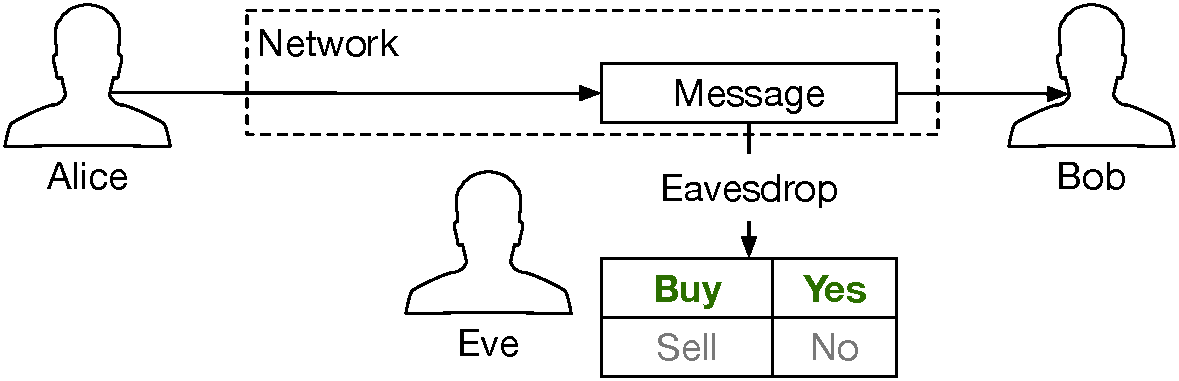
\includegraphics[width=85mm]{figures/confidentiality_attack.pdf}
  \caption{
    In a confidentiality attack, Eve sees the message sent by Alice to Bob and
    can understand the information inside it. In this case, Eve can tell that
    the message is a \textbf{buy} order, and not a \textbf{sell} order.
  }
  \label{fig:confidentiality_attack}
\end{figure}

A system with integrity guarantees would prevent Eve from replacing Alice's
message with a false order, as shown in Figure~\ref{fig:integrity_attack}. In
this example, without integrity guarantees, Eve could replace Alice's message
with a \textsc{sell-everything} order, and buy Alice's assets at a very low
price.

\begin{figure}[hbt]
  \centering
  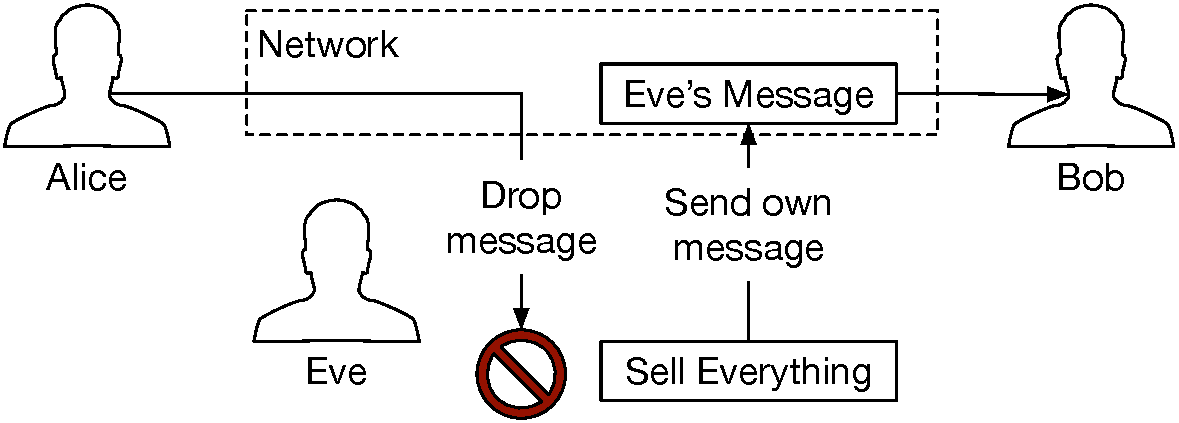
\includegraphics[width=85mm]{figures/integrity_attack.pdf}
  \caption{
    In an integrity attack, Eve replaces Alice's message with her own. In this
    case, Eve sends Bob a \textbf{sell-everything} order. In this case, Eve can
    tell that the message is a \textbf{buy} order, and not a \textbf{sell}
    order.
  }
  \label{fig:integrity_attack}
\end{figure}

Last, a communication system that guarantees freshness would ensure that Eve
cannot perform the replay attack pictured in Figure~\ref{fig:freshness_attack},
where she would replace Alice's message with an older message. Without
freshness guarantees, Eve could mount the following attack, which bypasses both
confidentiality and integrity guarantees. Over a few days, Eve would copy and
store Alice's messages from the network. When an order would reach Bob, Eve
would observe the market and determine if the order was \textsc{buy} or
\textsc{sell}. After building up a database of messages labeled \textsc{buy} or
\textsc{sell}, Eve would replace Alice's message with an old message of her
choice.

\begin{figure}[hbt]
  \centering
  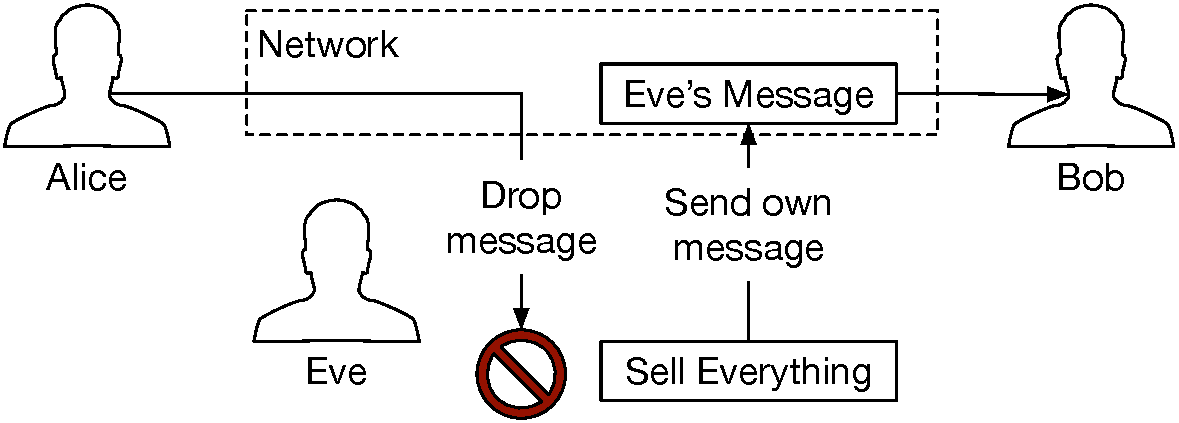
\includegraphics[width=85mm]{figures/integrity_attack.pdf}
  \caption{
    In a freshness attack, Eve replaces Alice's message with a message that she
    sent at an earlier time. In this example, Eve builds a database of labeled
    messages over time, and is able to send Bob her choice of a \textsc{buy} or
    a \textsc{sell} order.
  }
  \label{fig:freshness_attack}
\end{figure}


\HeadingLevelC{Cryptographic Keys}
\label{sec:crypto_keys}

All cryptographic primitives that we describe here rely on \textit{keys}, which
are small pieces of information that must only be disclosed according to
specific rules. A large part of a system's security analysis focuses on
ensuring that the keys used by the underlying cryptographic primitives are
produced and handled according to the primitives' assumptions.

Each cryptographic primitive has an associated \textit{key generation
algorithm} that uses random data to produce a unique key. The random data is
produced by a \textit{cryptographically strong pseudo-random number generator}
(CSPRNG) that expands a small amount of \textit{random seed} data into a much
larger amount of data, which is computationally indistinguishable from true
random data. The random seed must be obtained from a true source of randomness
whose output cannot be predicted by an adversary, such as the least significant
bits of the temperature readings coming from a hardware sensor.

\textit{Symmetric key} cryptography requires that all the parties in the system
establish a shared \textit{secret key}, which is usually referred to as ``the
key''. Typically, one party executes the key generation algorithm and securely
transmits the resulting key to the other parties, as illustrated in
Figure~\ref{fig:symmetric_key_generation}. The channel used to distribute the
key must provide confidentiality and integrity guarantees, which is a
non-trivial logistical burden. The symmetric key primitives mentioned here do
not make any assumption about the key, so the key generation algorithm simply
grabs a fixed number of bits from the CSPRNG.

\begin{figure}[hbt]
  \centering
  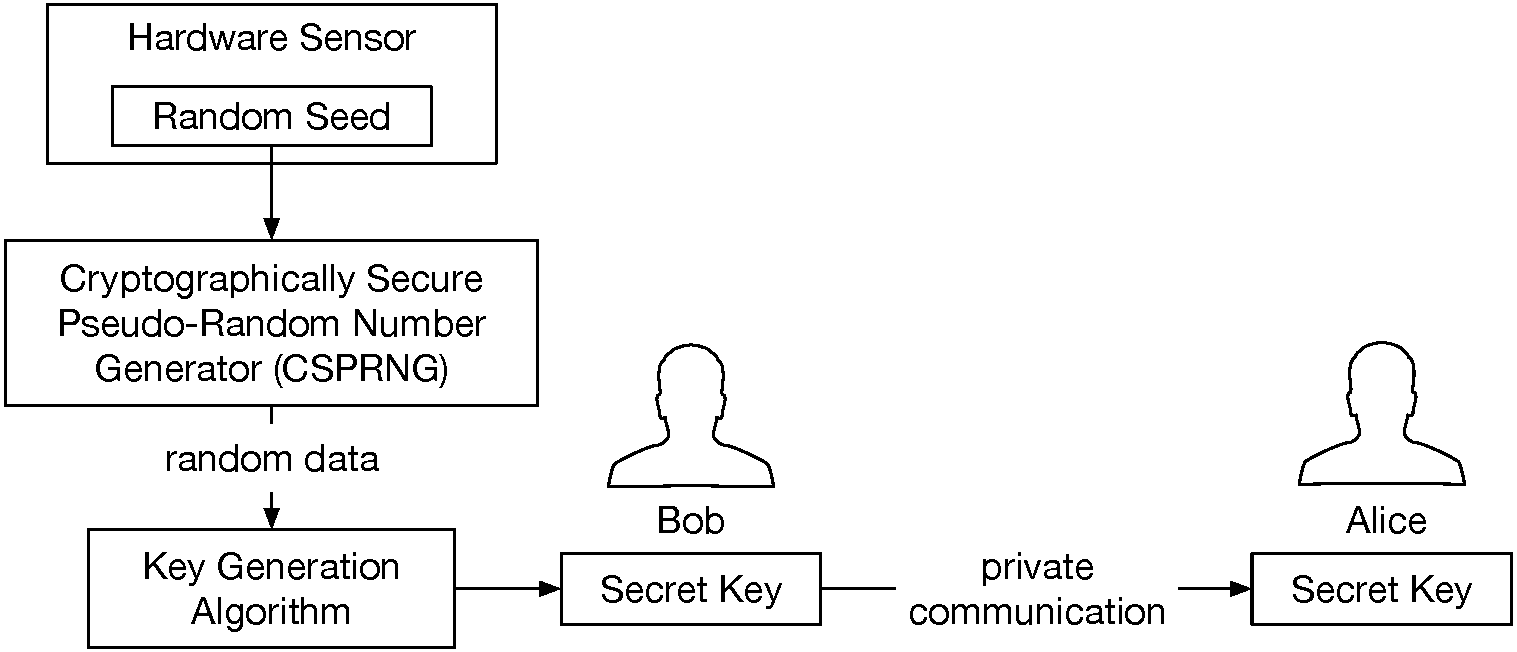
\includegraphics[width=87mm]{figures/symmetric_key_generation.pdf}
  \caption{
    In symmetric key cryptography, a secret key is shared by the parties that
    wish to communicate securely.
  }
  \label{fig:symmetric_key_generation}
\end{figure}

The defining feature of \textit{asymmetric key} cryptography is that it does
not require a private channel for key distribution. Each party executes the key
generation algorithm, which produces a \textit{private key} and a
\textit{public key} that are mathematically related. Each party's public key is
distributed to the other parties over a channel with integrity guarantees, as
shown in Figure~\ref{fig:asymmetric_key_generation}.  Asymmetric key primitives
are more flexible than their symmetric counterparts, but are more complicated
and consume more computational resources.

\begin{figure}[hbt]
  \centering
  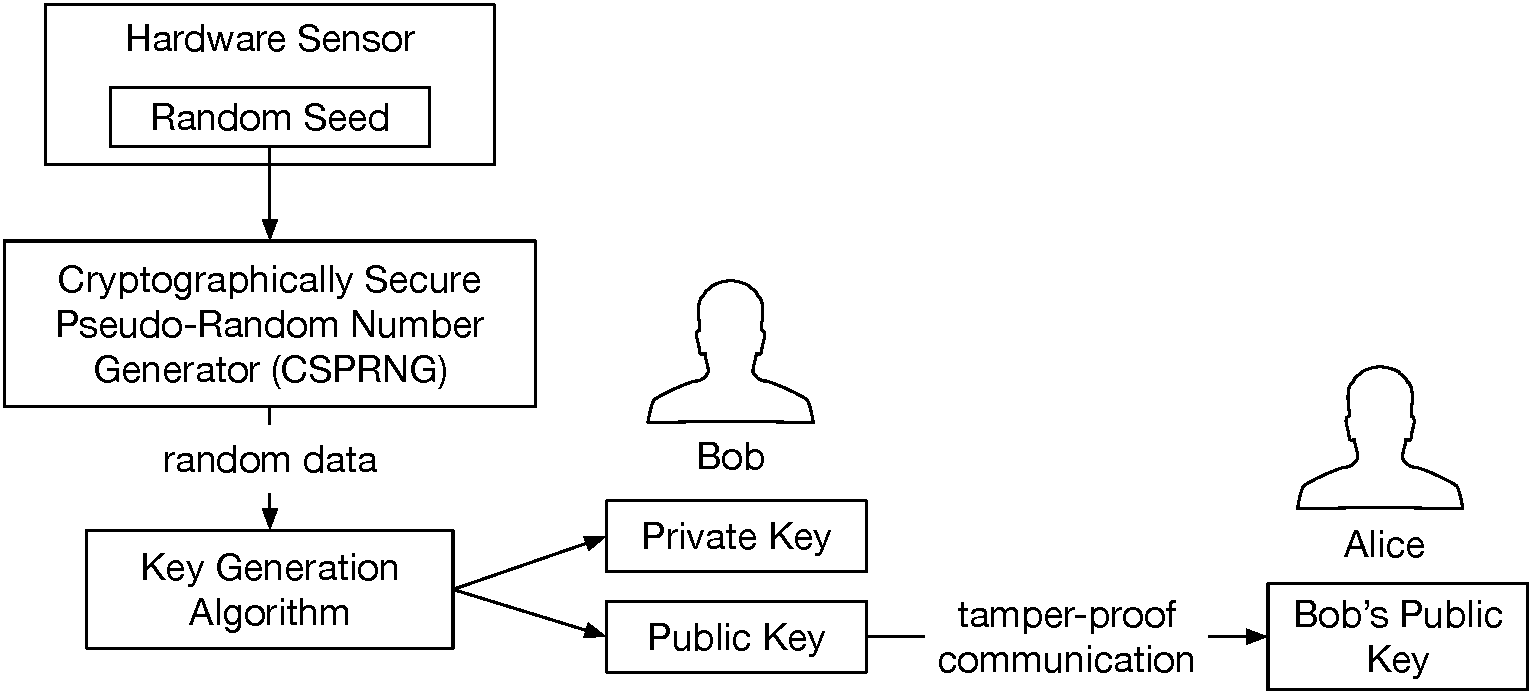
\includegraphics[width=87mm]{figures/asymmetric_key_generation.pdf}
  \caption{
    An asymmetric key generation algorithm produces a private key and an
    associated public key. The private key is held confidential, while the
    public key is given to any party who wishes to securely communicate with
    the private key's holder.
  }
  \label{fig:asymmetric_key_generation}
\end{figure}


\HeadingLevelC{Confidentiality}
\label{sec:confidentiality_crypto}

Many cryptosystems that provide integrity guarantees are built upon
\textit{block ciphers} that operate on fixed-size message blocks. The sender
transforms a block using an \textit{encryption} algorithm, and the receiver
inverts the transformation using a \textit{decryption} algorithm. The
encryption algorithms in block ciphers obfuscate the message block's content in
the output, so that an adversary who does not have the decryption key cannot
obtain the original message block from the encrypted output.

Symmetric key encryption algorithms use the same secret key for encryption and
decryption, as shown in Figure~\ref{fig:symmetric_block_cipher}, while
asymmetric key block ciphers use the public key for encryption, and the
corresponding private key for decryption, as shown in
Figure~\ref{fig:asymmetric_block_cipher}.
\begin{figure}[hbt]
  \centering
  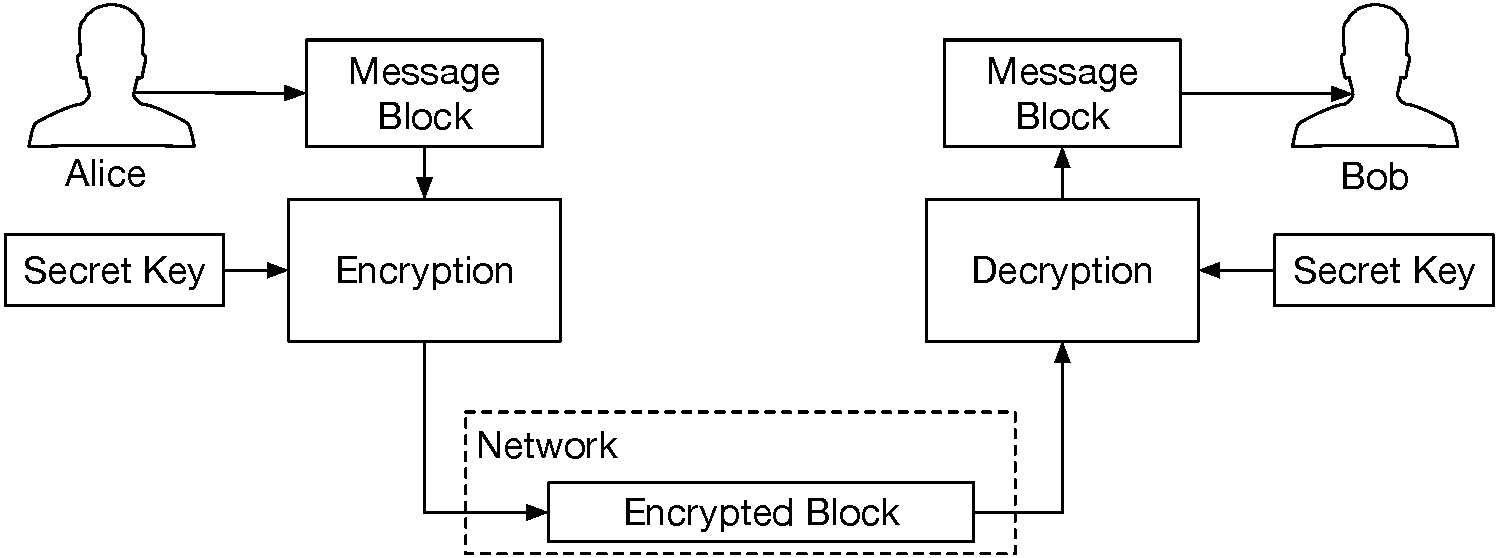
\includegraphics[width=85mm]{figures/symmetric_block_cipher.pdf}
  \caption{
    In a symmetric key secure permutation (block cipher), the same secret key
    must be provided to both the encryption and the decryption algorithm.
  }
  \label{fig:symmetric_block_cipher}
\end{figure}

\begin{figure}[hbt]
  \centering
  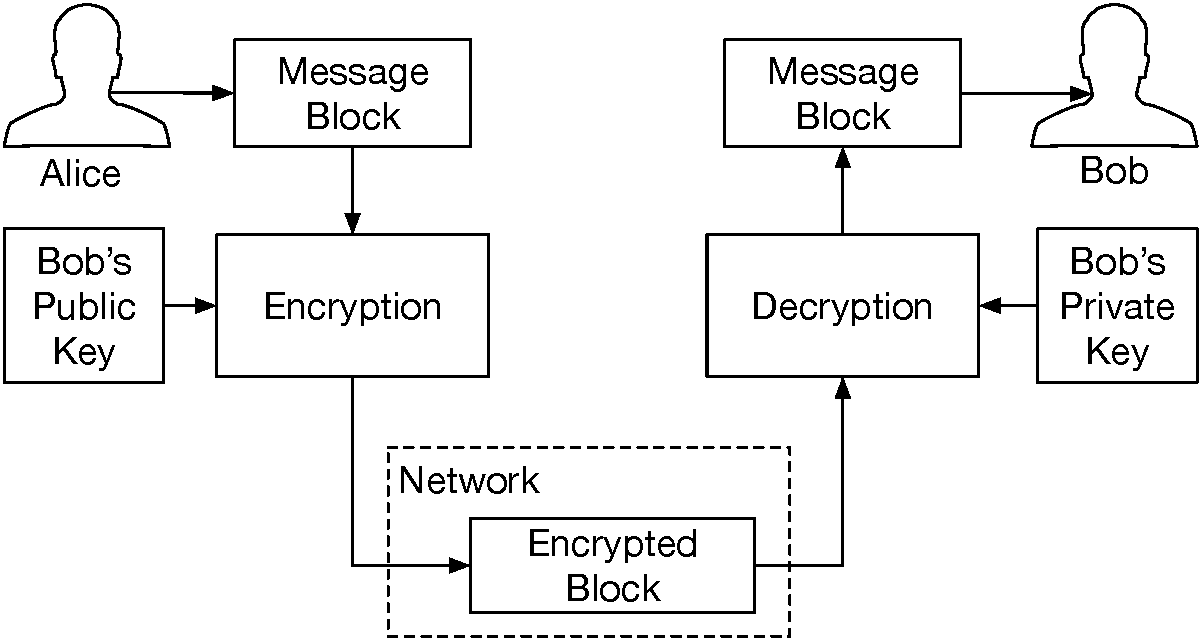
\includegraphics[width=85mm]{figures/asymmetric_block_cipher.pdf}
  \caption{
    In an asymmetric key block cipher, the encryption algorithm operates on a
    public key, and the decryption algorithm uses the corresponding private
    key.
  }
  \label{fig:asymmetric_block_cipher}
\end{figure}

The most popular block cipher based on symmetric keys at the time of this
writing is the
\textit{American Encryption Standard}~(AES)~\cite{daemen1999aes, fips2001aes},
with two variants that operate on 128-bit blocks using 128-bit keys or 256-bit
keys. AES is a \textit{secure permutation} function, as it can transform any
128-bit block into another 128-bit block. Recently, the United States
\textit{National Security Agency}~(NSA) required the use of 256-bit AES keys
for protecting sensitive information~\cite{nsa2015suiteb}.

The most deployed asymmetric key block cipher is the
\textit{Rivest-Shamir-Adelman}~(RSA)~\cite{rivest1978rsa} algorithm. RSA has
variable key sizes, and 3072-bit key pairs are considered to provide the same
security as 128-bit AES keys~\cite{fips2012keysize}.

A block cipher does not necessarily guarantee confidentiality, when used on its
own.  A noticeable issue is that in our previous example, a block cipher would
generate the same encrypted output for any of Alice's \textsc{buy} orders, as
they all have the same content. Furthermore, each block cipher has its own
assumptions that can lead to subtle vulnerabilities if the cipher is used
directly.

Symmetric key block ciphers are combined with operating modes to form symmetric
encryption schemes. Most operating modes require a random
\textit{initialization vector} (IV) to be used for each message, as shown in
Figure~\ref{fig:symmetric_encryption}. When analyzing the security of systems
based on these cryptosystems, an understanding of the IV generation process is
as important as ensuring the confidentiality of the encryption key.

\begin{figure}[hbt]
  \centering
  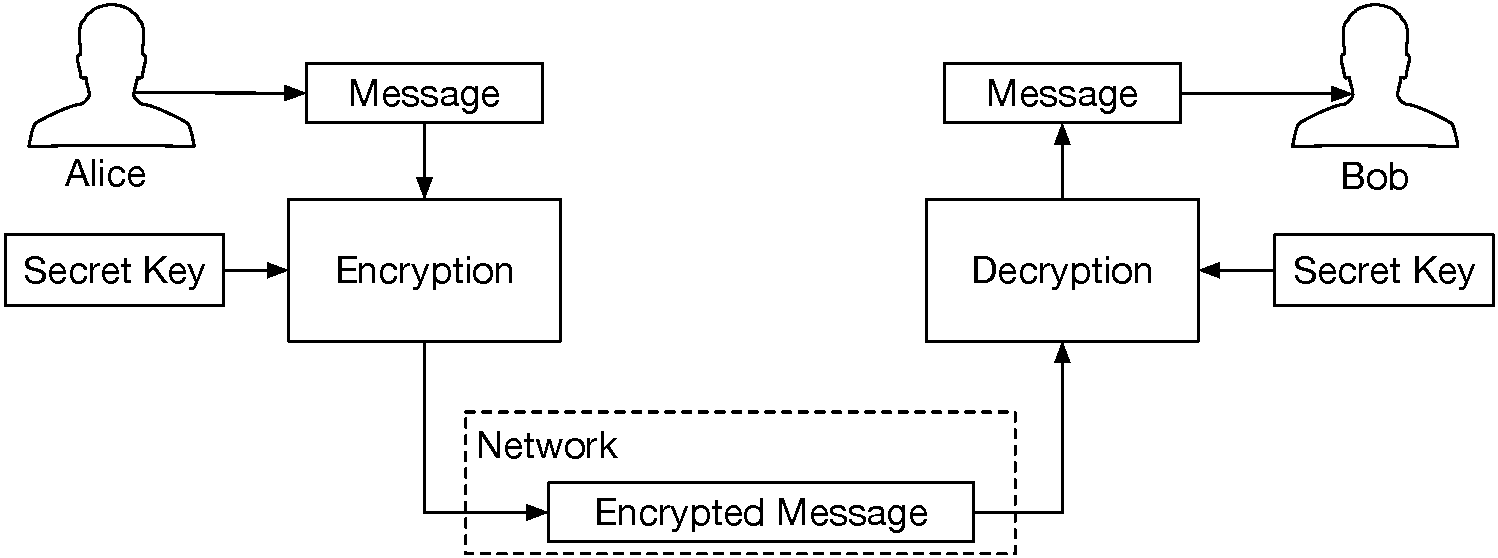
\includegraphics[width=85mm]{figures/symmetric_encryption.pdf}
  \caption{
    Symmetric key block ciphers are combined with operating modes. Most
    operating modes require a random initialization vector (IV) to be generated
    for each encrypted message.
  }
  \label{fig:symmetric_encryption}
\end{figure}

Counter (CTR) and Cipher Block Chaining (CBC) are examples of operating modes
recommended~\cite{fips2001ctr} by the United States \textit{National Institute
of Standards and Technology}~(NIST), which informs the NSA's requirements.
Combining a block cipher, such as AES, with an operating mode, such as CTR,
results in an encryption method, such as AES-CTR, which can be used to add
confidentiality guarantees.

In the asymmetric key setting, there is no concept equivalent to operating
modes. Each block cipher has its own assumptions, and requires a specialized
scheme for general-purpose usage.

The RSA algorithm is used in conjunction with \textit{padding methods}, the
most popular of which are the methods described in the \textit{Public-Key
Cryptography Standard} (PKCS) \#1 versions 1.5~\cite{kaliski1998pkcs1v15} and
2.0~\cite{kaliski1998pkcs1v2}. A security analysis of a system that uses
RSA-based encryption must take the padding method into consideration. For
example, the padding in PKCS \#1 v1.5 can leak the private key under certain
circumstances~\cite{bleichenbacher1998pkcs1v15cca}. While PKCS \#1 v2.0 solves
this issue, it is complex enough that some implementations have their own
security issues~\cite{manger2001pkcs1v20attack}.

Asymmetric encryption algorithms have much higher computational requirements
than symmetric encryption algorithms. Therefore, when non-trivial quantities of
data is encrypted, the sender generates a single-use secret key that is used
to encrypt the data, and encrypts the secret key with the receiver's public
key, as shown in Figure~\ref{fig:asymmetric_encryption}.

\begin{figure}[hbt]
  \centering
  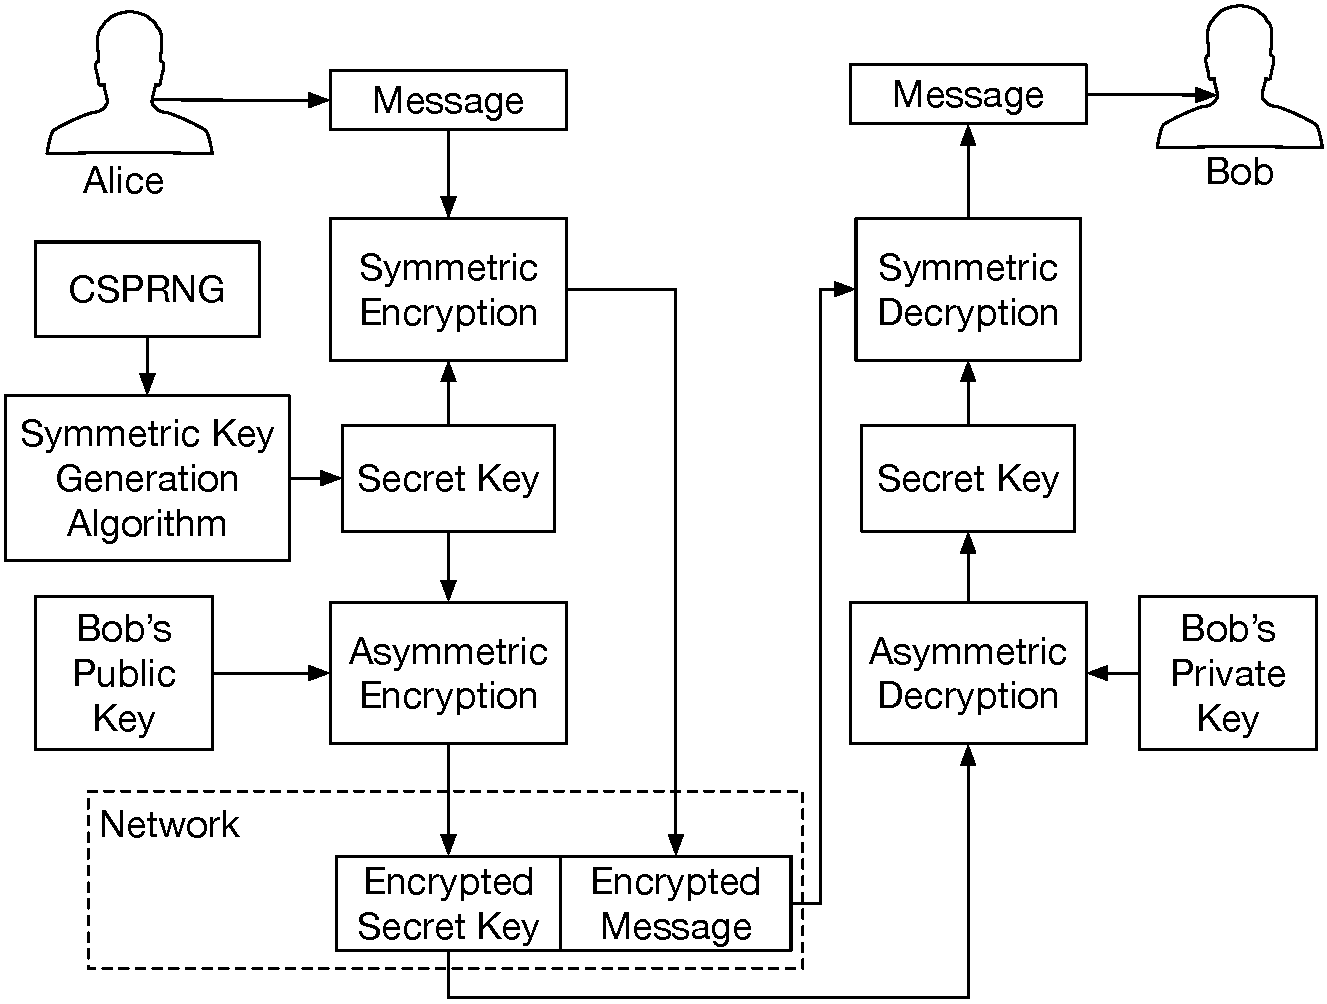
\includegraphics[width=87mm]{figures/asymmetric_encryption.pdf}
  \caption{
    Asymmetric key encryption is generally used to bootstrap a symmetric
    key encryption scheme.
  }
  \label{fig:asymmetric_encryption}
\end{figure}


\HeadingLevelC{Integrity}
\label{sec:integrity_crypto}

Many cryptosystems that provide integrity guarantees are built upon
\textit{secure hashing} functions. These hash functions operate on an unbounded
amount of input data and produce a small fixed-size output. Secure hash
functions have a few guarantees, such as \textit{pre-image resistance}, which
states that an adversary cannot produce input data corresponding to a given
hash output.

At the time of this writing, the most popular secure hashing function is the
\textit{Secure Hashing Algorithm}~(SHA)~\cite{eastlake2001sha1}. However, due
to security issues in SHA-1~\cite{stevens2015sha1attack}, new software is
recommended to use at least 256-bit SHA-2~\cite{fips2015shs} for secure
hashing.

The SHA hash functions are members of a large family of \textit{block hash
functions} that consume their input in fixed-size message blocks, and use a
fixed-size internal state. A block hash function is used as shown in
Figure~\ref{fig:block_hash_operation}. An \textsc{initialize} algorithm is
first invoked to set the internal state to its initial values. An
\textsc{extend} algorithm is executed for each message block in the input.
After the entire input is consumed, a \textsc{finalize} algorithm produces the
hash output from the internal state.

\begin{figure}[hbt]
  \centering
  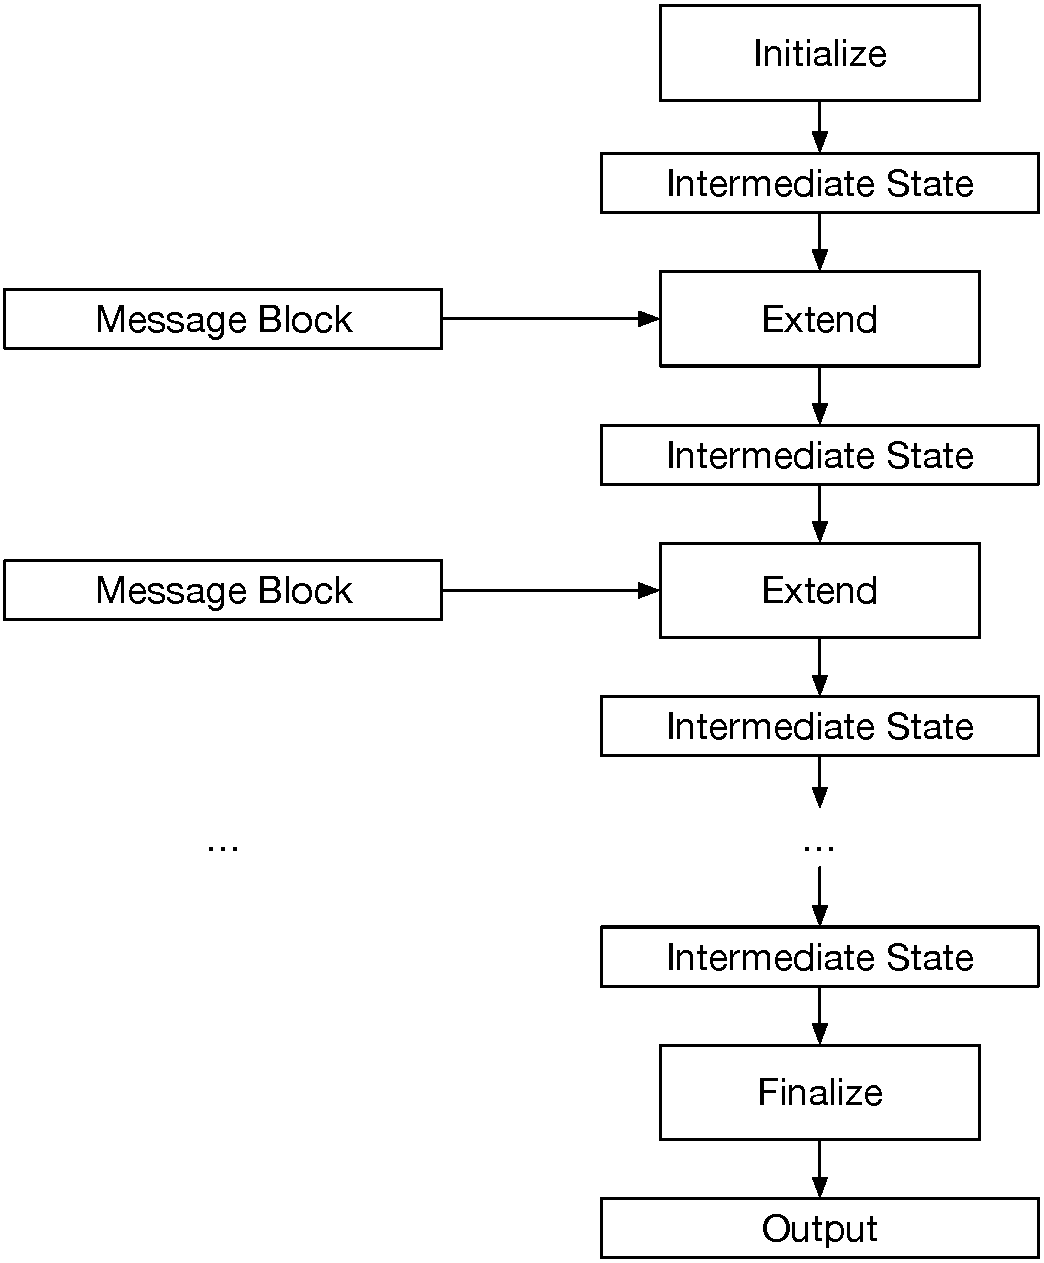
\includegraphics[width=70mm]{figures/block_hash_operation.pdf}
  \caption{
    A block hash function operates on fixed-size message blocks and uses a
    fixed-size internal state.
  }
  \label{fig:block_hash_operation}
\end{figure}

In the symmetric key setting, integrity guarantees are obtained using a
\textit{Message Authentication Code}~(MAC) cryptosystem, illustrated in
Figure~\ref{fig:symmetric_mac}. The sender uses a MAC algorithm that reads in a
symmetric key and a variable-legnth message, and produces a fixed-length, short
\textit{MAC tag}. The receiver provides the original message, the symmetric
key, and the MAC tag to a MAC verification algorithm that checks the
authenticity of the message.

\begin{figure}[hbt]
  \centering
  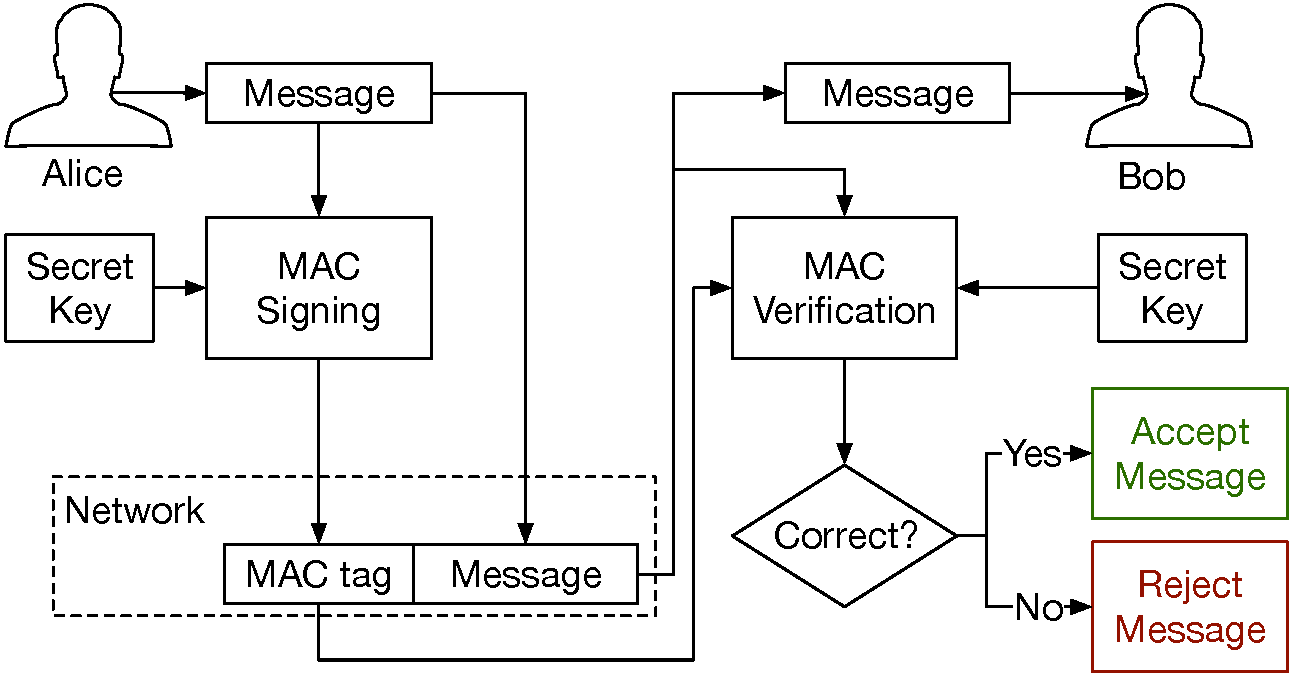
\includegraphics[width=87mm]{figures/symmetric_mac.pdf}
  \caption{
    In the symmetric key setting, integrity is assured by computing a
    Message Authentication Code (MAC) tag and transmitting it over the network
    along the message. The receiver feeds the MAC tag into a verification
    algorithm that checks the message's authenticity.
  }
  \label{fig:symmetric_mac}
\end{figure}

The key property of MAC cryptosystems is that an adversary cannot produce a
MAC tag that will validate a message without the secret key.

Many MAC cryptosystems do not have a separate MAC verification algorithm.
Instead, the receiver checks the authenticity of the MAC tag by running the
same algorithm as the sender to compute the expected MAC tag for the received
message, and compares the output with the MAC tag received from the network.

This is the case for the
\textit{Hash Message Authentication Code}~(HMAC)~\cite{krawczyk1997hmac}
generic construction, whose operation is illustrated in
Figure~\ref{fig:symmetric_hmac}. HMAC can use any secure hash function, such as
SHA, to build a MAC cryptosystem.

\begin{figure}[hbt]
  \centering
  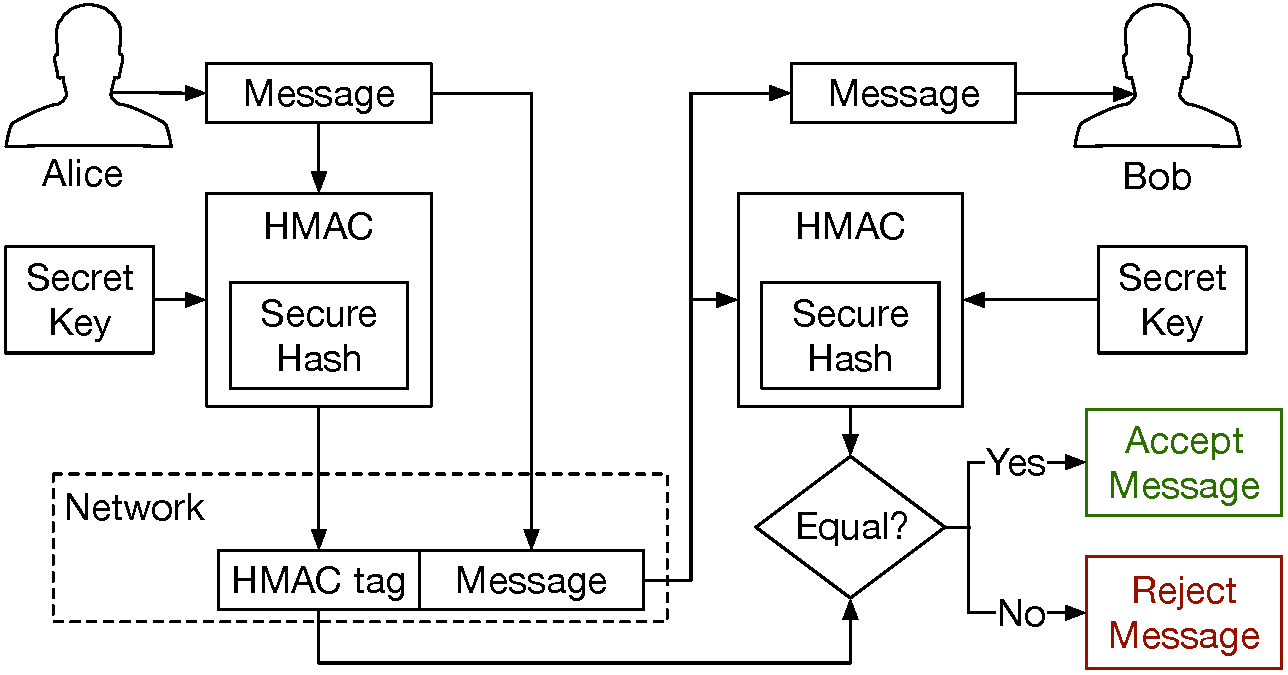
\includegraphics[width=87mm]{figures/symmetric_hmac.pdf}
  \caption{
    In the symmetric key setting, integrity is assured by computing a
    Hash-bassed Message Authentication Code (HMAC) and transmitting it over the
    network along the message. The receiver re-computes the HMAC and compares
    it against the version received from the network.
  }
  \label{fig:symmetric_hmac}
\end{figure}

Asymmetric key primitives that provide integrity guarantees are known as
\textit{signatures}. The message sender provides her private key to a
\textit{signing} algorithm, and transmits the output signature along with the
message, as shown in Figure~\ref{fig:asymmetric_signing}. The message receiver
feeds the sender's public key and the signature to a \textit{signature
verification} algorithm, which returns \textsc{true} if the message matches the
signature, and \textsc{false} if the message has been tampered with.

\begin{figure}[hbt]
  \centering
  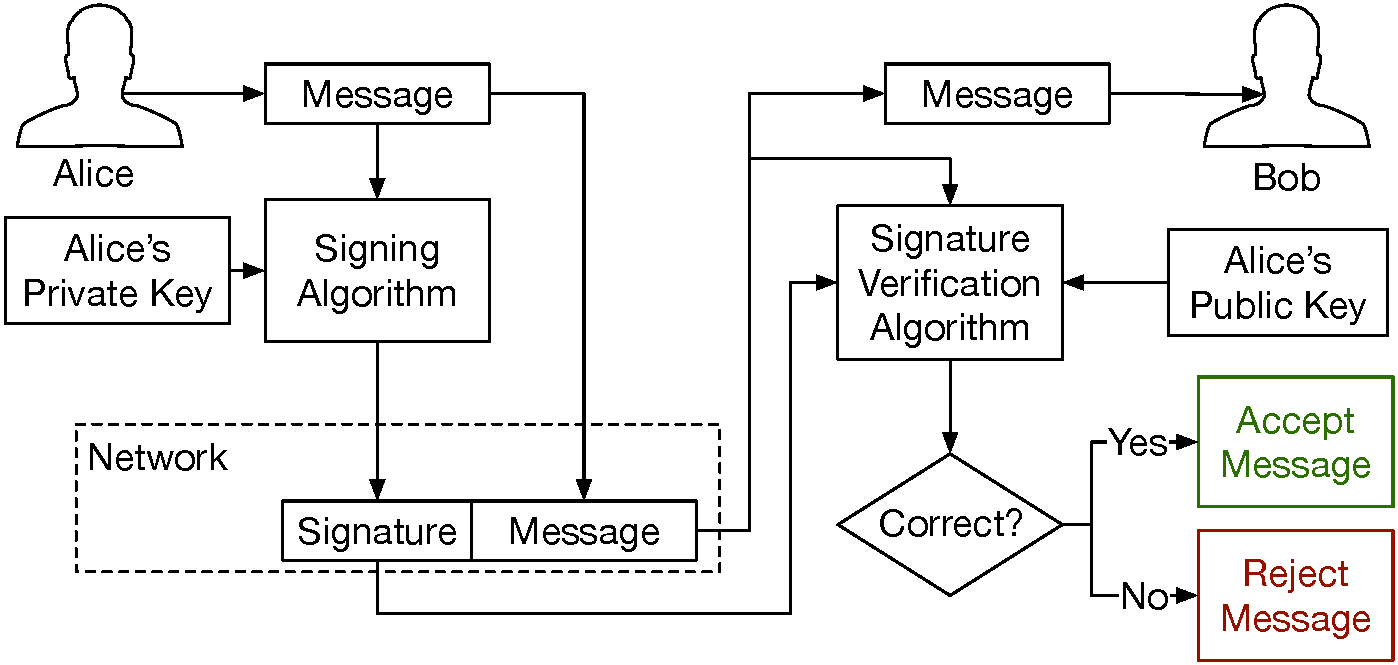
\includegraphics[width=87mm]{figures/asymmetric_signing.pdf}
  \caption{
    Signature schemes guarantee integrity in the asymmetric key setting.
    Signatures are created using the sender's private key, and are verified
    using the corresponding public key. A cryptographically secure hash
    function is usually employed to reduce large messages to small hashes,
    which are then signed.
  }
  \label{fig:asymmetric_signing}
\end{figure}

Signing algorithms can only operate on small messages and are computationally
expensive. Therefore, in practice, the message to be transmitted is first ran
through a cryptographically strong hash function, and the hash is provided as
the input to the signing algorithm.

At the time of this writing, the most popular choice for guaranteeing integrity
in shared secret settings is HMAC-SHA, an HMAC function that uses SHA for
hashing.

\textit{Authenticated encryption}, which combines a block cipher with an
operating mode that offers both confidentiality and integrity guarantees, is
often an attractive alternative to HMAC. The most popular authenticated
encryption operating mode is \textit{Galois/Counter operation
mode}~(GCM)~\cite{mcgrew2004gcm}, which has earned NIST's
recommendation~\cite{fips2017gcm} when combined with AES to form AES-GCM.

The most popular signature scheme combines the RSA encryption algorithms with a
padding schemes specified in PKCS \#1, as illustrated in
Figure~\ref{fig:rsa_pkcs1_v15_padding}. Recently, elliptic curve cryptography
(ECC)~\cite{koblitz1987ecc} has gained a surge in popularity, thanks to its
smaller key sizes. For example, a 384-bit ECC key is considered to be as secure
as a 3072-bit RSA key~\cite{fips2012keysize, nsa2015suiteb}. The NSA requires
the Digital Signature Standard~(DSS)\cite{fips2013dss}, which specifies schemes
based on RSA and ECC.

\begin{figure}[hbt]
  \centering
  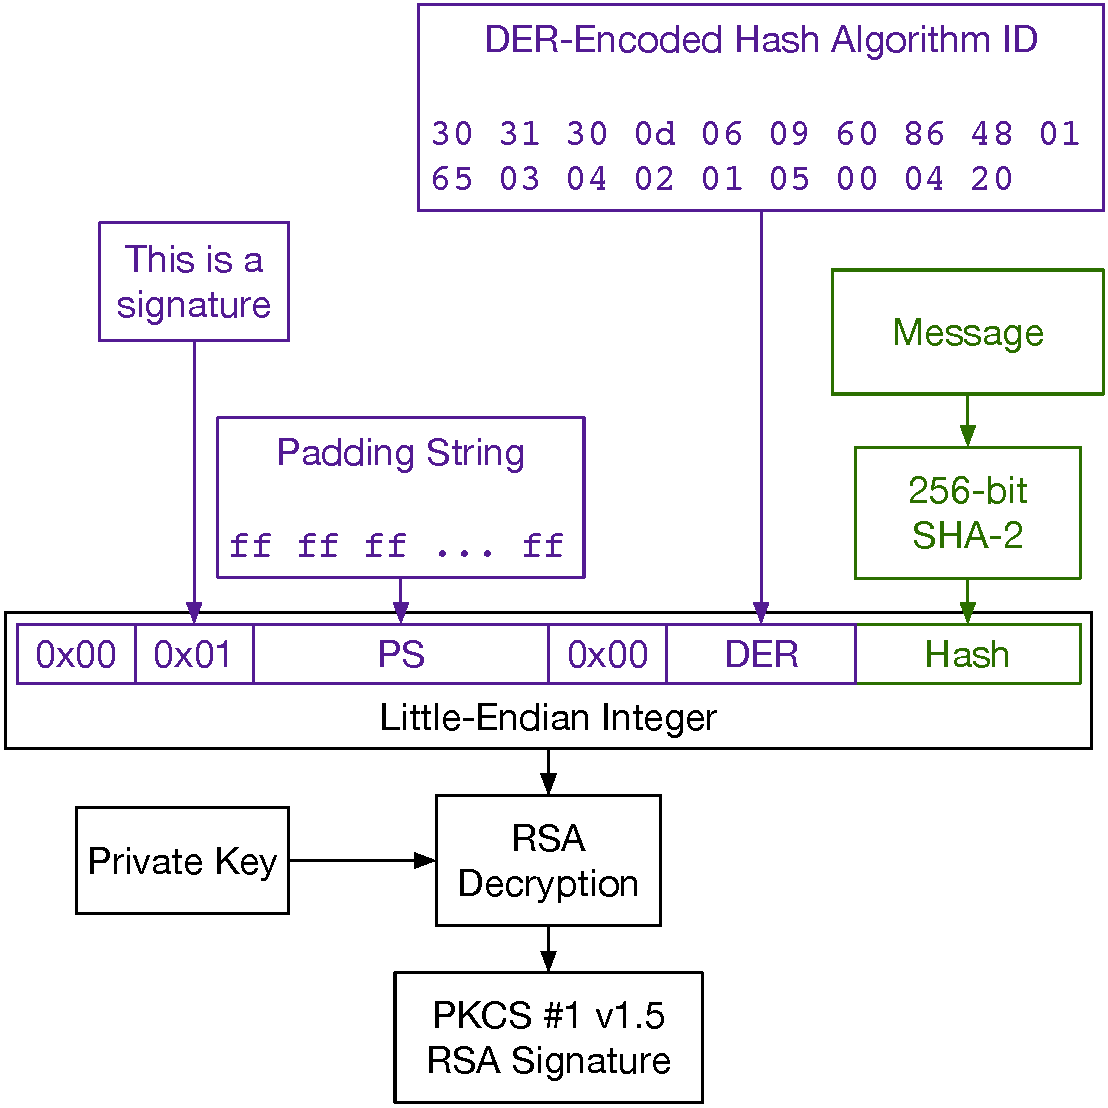
\includegraphics[width=85mm]{figures/rsa_pkcs1_v15_padding.pdf}
  \caption{
    The RSA signature scheme with PKCS \#1 v1.5 padding specified in RFC 3447
    combines a secure hash of the signed message with a DER-encoded
    specification of the secure hash algorithm used by the signature, and a
    padding string whose bits are all set to 1. Everything except for the
    secure hash output is considered to be a part of the PKCS \#1 v1.5 padding.
  }
  \label{fig:rsa_pkcs1_v15_padding}
\end{figure}


\HeadingLevelC{Freshness}
\label{sec:freshness_crypto}

Freshness guarantees are typically built on top of a system that already offers
integrity guarantees, by adding a unique piece of information to each message.
The main challenge in freshness schemes comes down to economically maintaining
the state needed to generate the unique pieces of information on the sender
side, and verify their uniqueness on the receiver side.

A popular solution for gaining freshness guarantees relies on \textit{nonces},
single-use random numbers. Nonces are attractive because the sender does not
need to maintain any state; the receiver, however, must store the nonces of all
received messages.

Nonces are often combined with a message timestamping and expiration scheme, as
shown in Figure~\ref{fig:timestamped_nonces}. An expiration can greatly reduce
the receiver's storage requirement, as the nonces for expired messages can be
safely discarded. However, the scheme depends on the sender and receiver having
synchronized clocks. The message expiration time is a compromise between the
desire to reduce storage costs, and the need to tolerate clock skew and delays
in message transmission and processing.

\begin{figure}[hbt]
  \centering
  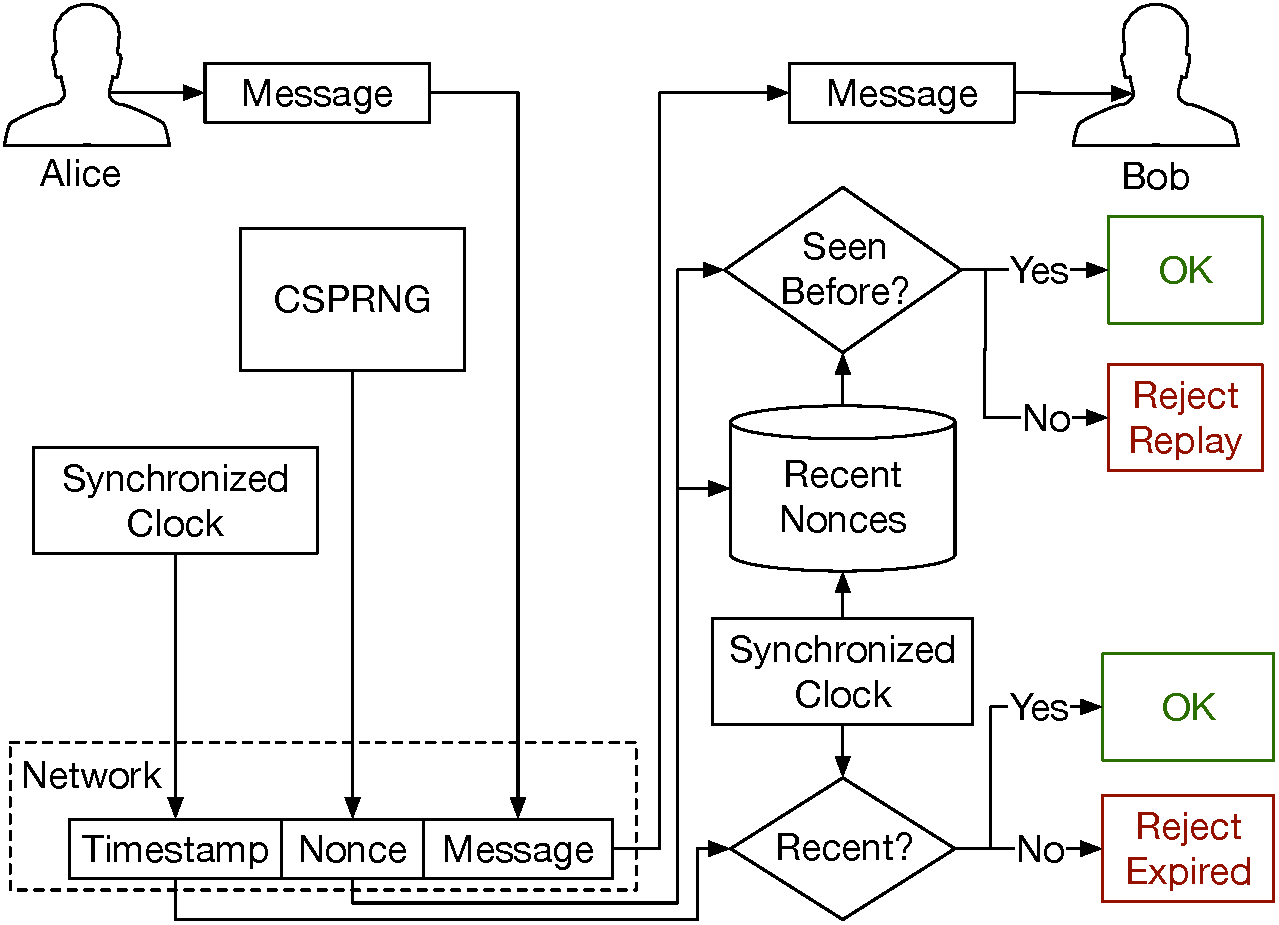
\includegraphics[width=87mm]{figures/timestamped_nonces.pdf}
  \caption{
    Freshness guarantees can be obtained by adding timestamped nonces on top
    of a system that already offers integrity guarantees. The sender and the
    receiver use synchronized clocks to timestamp each message and discard
    unreasonably old messages. The receiver must check the nonce in each new
    message against a database of the nonces in all the unexpired messages that
    it has seen.
  }
  \label{fig:timestamped_nonces}
\end{figure}

Alternatively, nonces can be used in challenge-response protocols, in a manner
that removes the storage overhead concerns. The challenger generates a nonce
and embeds it in the challenge message. The response to the challenge includes
an acknowledgement of the embedded nonce, so the challenger can distinguish
between a fresh response and a replay attack. The nonce is only stored by the
challenger, and is small in comparison to the rest of the state needed to
validate the response.

\subsection{Cryptographic Constructs}
\label{sec:crypto_constructs}

This section summarizes two constructs that are built on the cryptographic
primitives described in \S~\ref{sec:crypto_primitives}, and are used in the
rest of this work.


\subsubsection{Certificate Authorities}
\label{sec:certificates}

Asymmetric key cryptographic primitives assume that each party has the correct
public keys for the other parties. This assumption is critical, as the entire
security argument of an asymmetric key system rests on the fact that certain
operations can only be performed by the owners of the private keys
corresponding to the public keys. More concretely, if Eve can convince Bob
that her own public key belongs to Alice, Eve can produce message signatures
that seem to come from Alice.

The introductory material in \S~\ref{sec:crypto_primitives} assumed that each
party transmits its public key over a channel with integrity guarantees. In
practice, this is not a reasonable assumption, and the secure distribution of
public keys is still an open research problem.

The most widespread solution to the public key distribution problem is the
Certificate Authority (CA) system, which assumes the existence of a trusted
authority whose public key is securely transmitted to all the other parties in
the system.

The CA is responsible for securely obtaining the public key of each party, and
for issuing a \textit{certificate} that binds a party's identity (e.g.,
``Alice'') to its public key, as shown in Figure~\ref{fig:certificate}.

\begin{figure}[hbt]
  \centering
  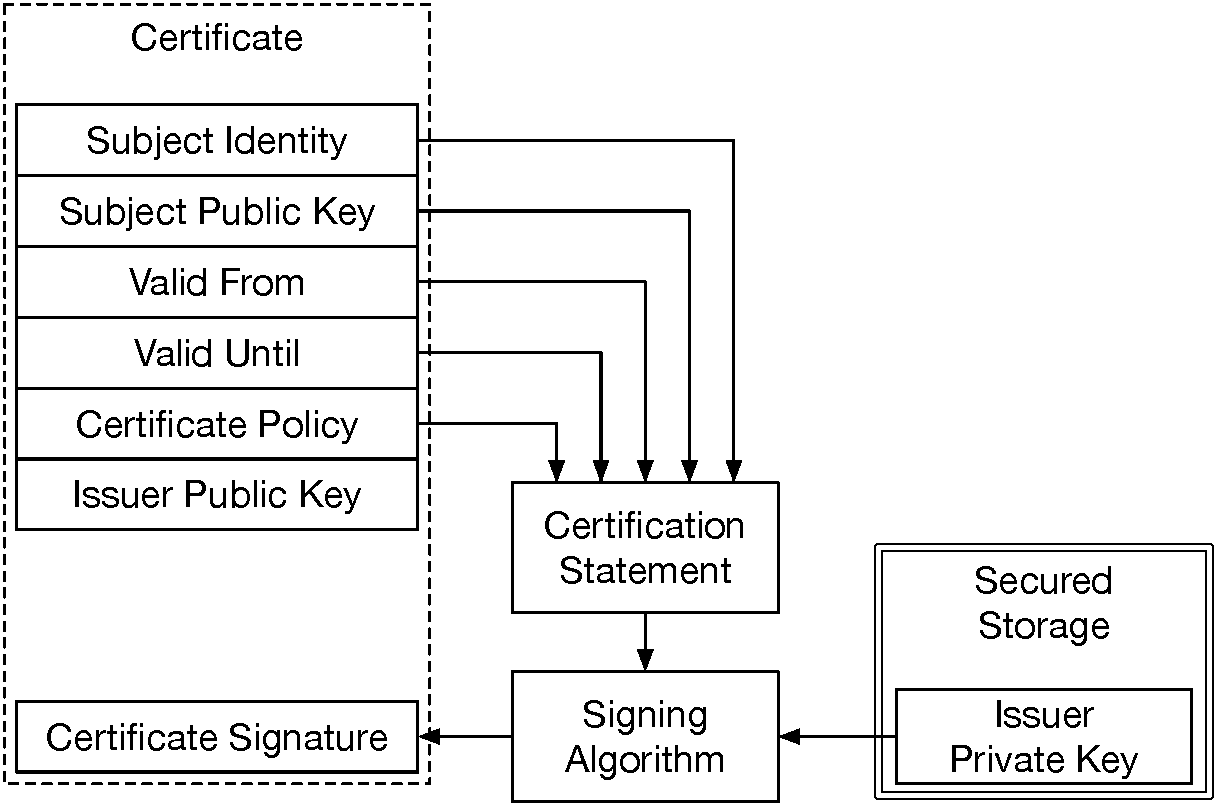
\includegraphics[width=85mm]{figures/certificate.pdf}
  \caption{
    A certificate is a statement signed by a certificate authority (issuer)
    binding the identity of a subject to a public key.
  }
  \label{fig:certificate}
\end{figure}

A certificate is essentially a cryptographic signature produced by the private
key of the certificate's \textit{issuer}, who is generally a CA. The message
signed by the issuer states that a public key belongs to a \textit{subject}.
The certificate message generally contains identifiers that state the intended
use of the certificate, such as ``the key in this certificate can only be used
to sign e-mail messages''. The certificate message usually also includes an
identifier for the issuer's \textit{certification policy}, which summarizes the
means taken by the issuer to ensure the authenticity of the subject's public
key.

A major issue in a CA system is that there is no obvious way to revoke a
certificate. A revocation mechanism is desirable to handle situations where a
party's private key is accidentally exposed, to avoid having an attacker use
the certificate to impersonate the compromised party. While advanced systems
for certificate revocation have been developed, the first line of defense
against key compromise is adding expiration dates to certificates.

In a CA system, each party presents its certificate along with its public key.
Any party that trusts the CA and has obtained the CA's public key securely can
verify any certificate using the process illustrated in
Figure~\ref{fig:certificate_validation}.

\begin{figure}[hbt]
  \centering
  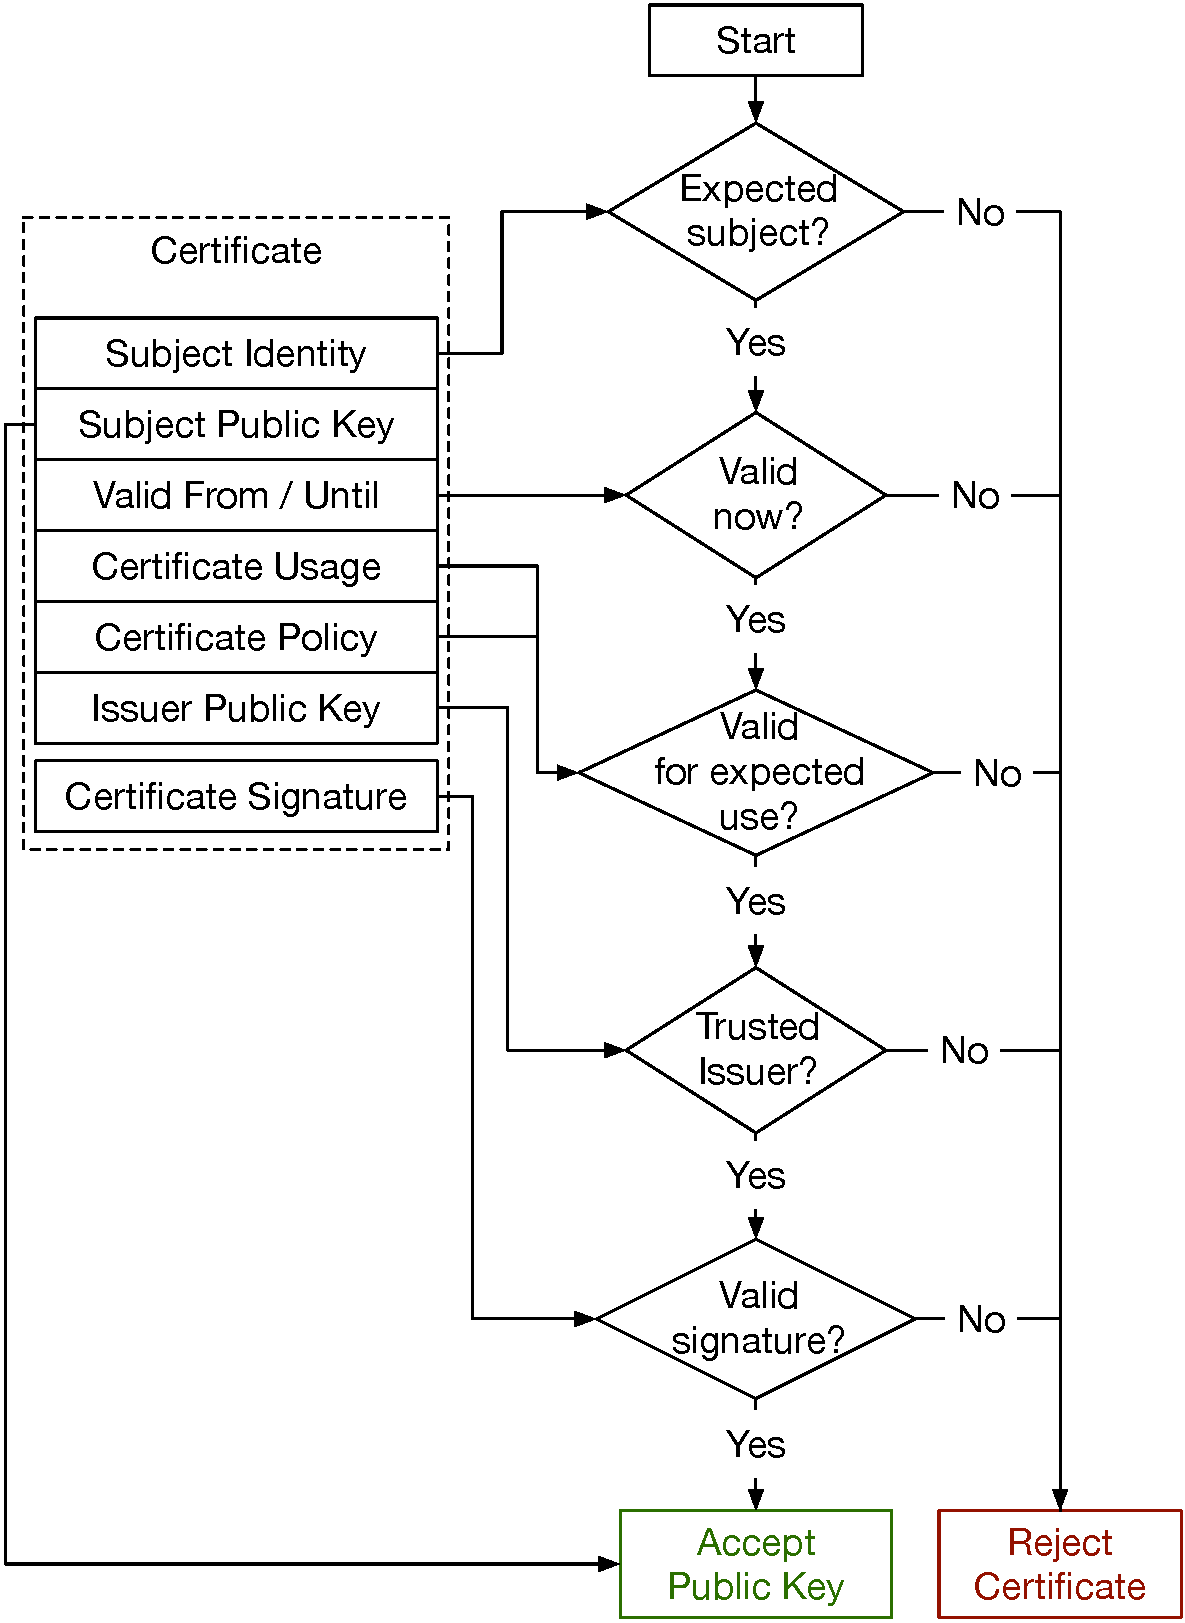
\includegraphics[width=80mm]{figures/certificate_validation.pdf}
  \caption{
    A certificate issued by a CA can be validated by any party that has
    securely obtained the CA's public key. If the certificate is valid, the
    subject public key contained within can be trusted to belong to the subject
    identified by the certificate.
  }
  \label{fig:certificate_validation}
\end{figure}

One of the main drawbacks of the CA system is that the CA's private key becomes
a very attractive attack target. This issue is somewhat mitigated by minimizing
the use of the CA's private key, which reduces the opportunities for its
compromise. The authority described above becomes the \textit{root CA}, and its
private key is only used to produce certificates for the
\textit{intermediate CAs} which, in turn, are responsible for generating
certificates for the other parties in the system, as shown in
Figure~\ref{fig:intermediate_cas}.

\begin{figure}[hbtp]
  \centering
  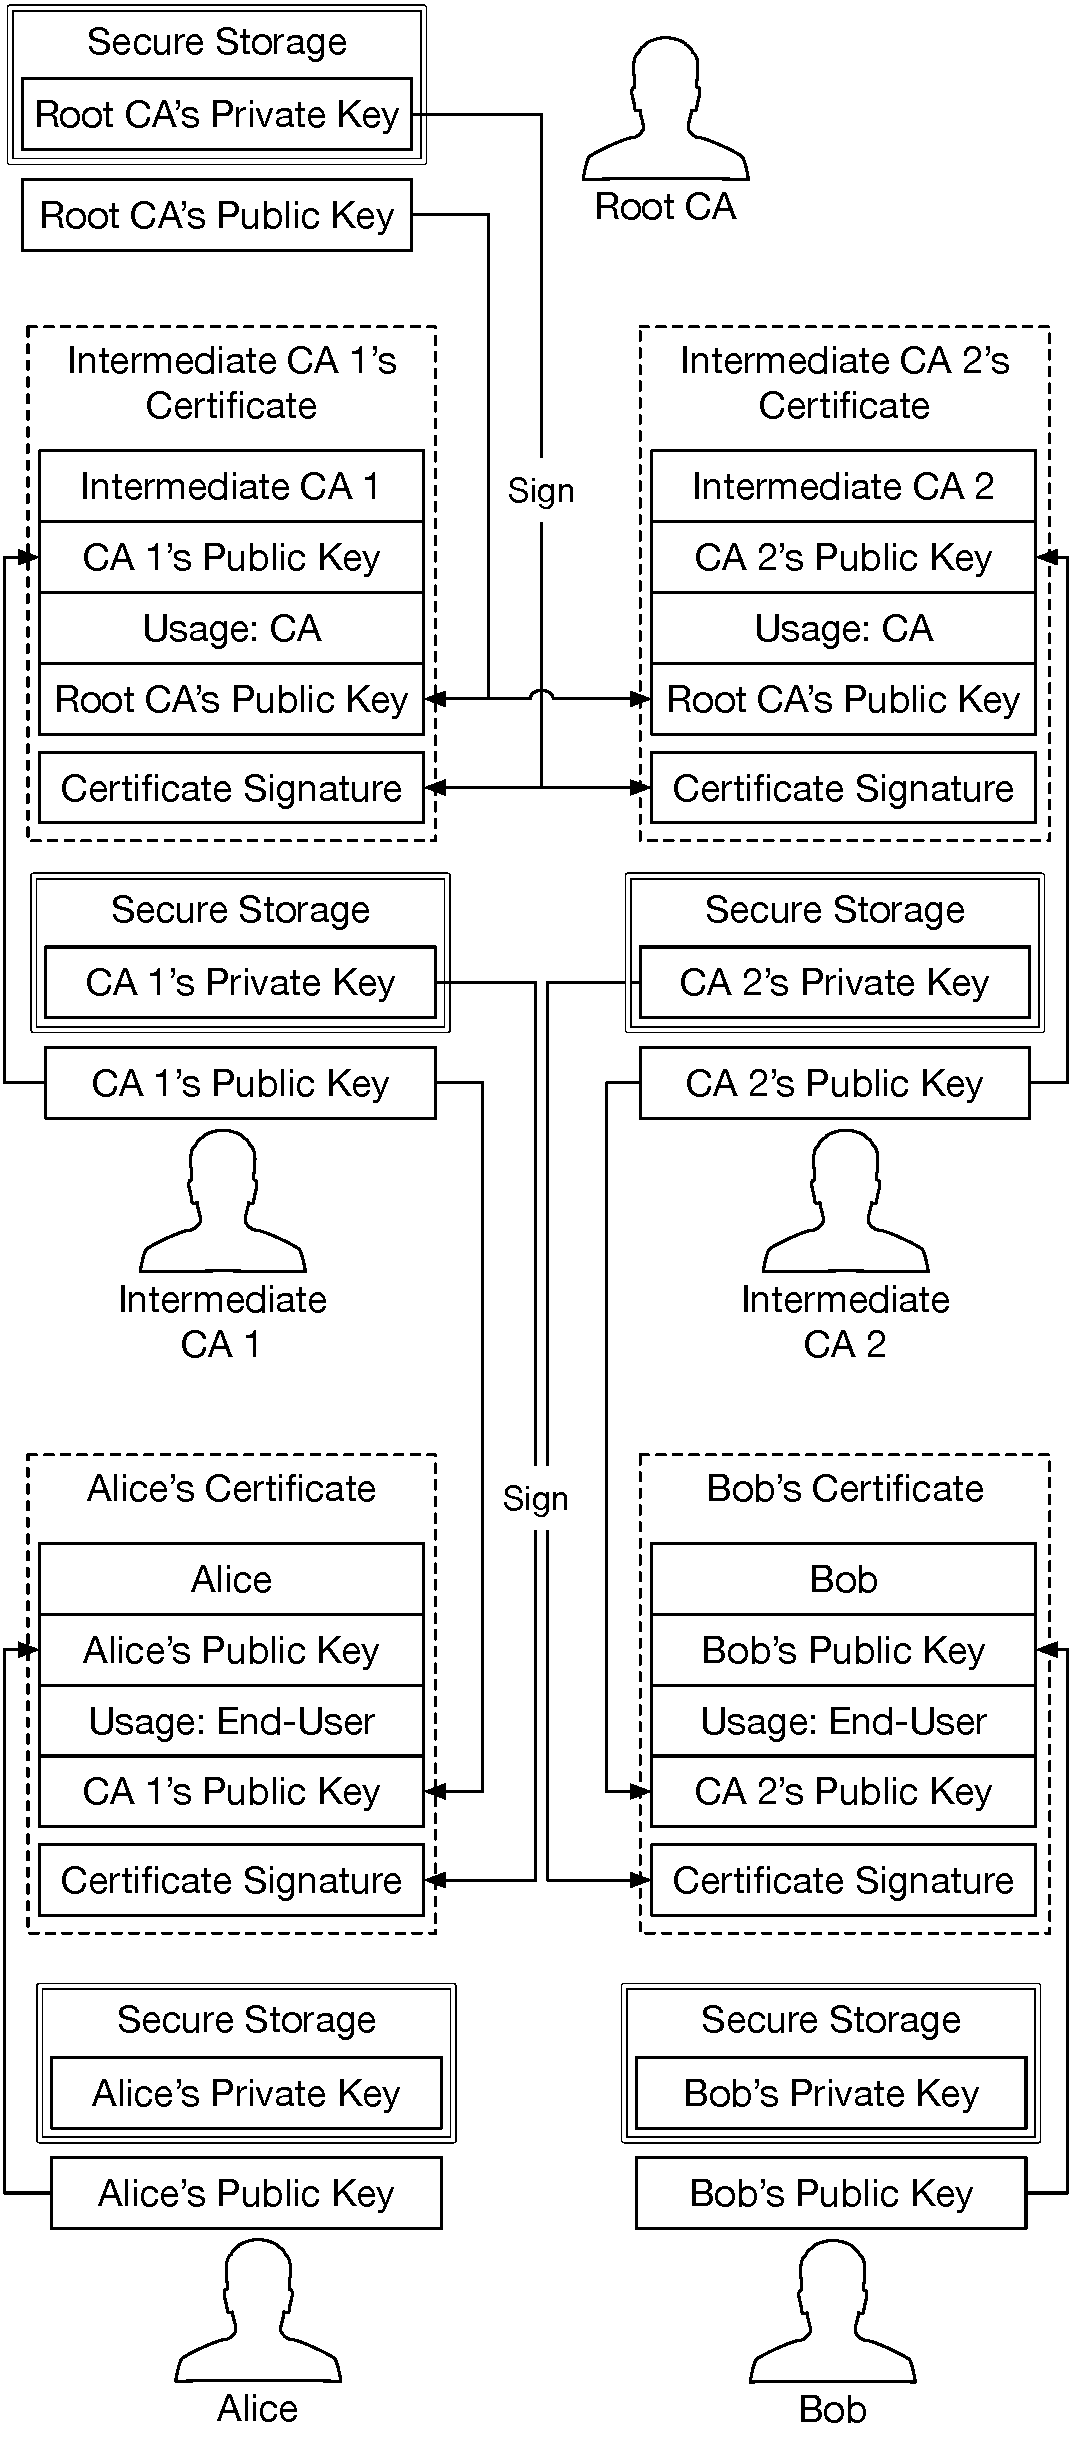
\includegraphics[width=75mm]{figures/intermediate_cas.pdf}
  \caption{
    A hierarchical CA structure minimizes the usage of the root CA's private
    key, reducing the opportunities for it to get compromised. The root CA only
    signs the certificates of intermediate CAs, which sign the end users'
    certificates.
  }
  \label{fig:intermediate_cas}
\end{figure}

In hierarchical CA systems, the only public key that gets distributed securely
to all the parties is the root CA's public key. Therefore, when two parties
wish to interact, each party must present its own certificate, as well as the
certificate of the issuing CA. For example, given the hierarchy in
Figure~\ref{fig:intermediate_cas}, Alice would prove the authenticity of her
public key to Bob by presenting her certificate, as well as the certificate of
Intermediate CA 1. Bob would first use the steps in
Figure~\ref{fig:certificate_validation} to validate Intermediate CA 1's
certificate against the root CA's public key, which would assure him of the
authenticity of Intermediate CA 1's public key. Bob would then validate Alice's
certificate using Intermediate CA 1's public key, which he now trusts.

In most countries, the government issues ID cards for its citizens, and
therefore acts as as a certificate authority. An ID card, shown in
Figure~\ref{fig:id_card_as_certificate}, is a certificate that binds a
subject's identity, which is a full legal name, to the subject's physical
appearance, which is used as a public key.

The CA system is very similar to the identity document (also known as ID card)
systems used to establish a person's identity, and a comparison between the two
may help further the reader's understanding of the concepts in the CA system.

\begin{figure}[hbt]
  \centering
  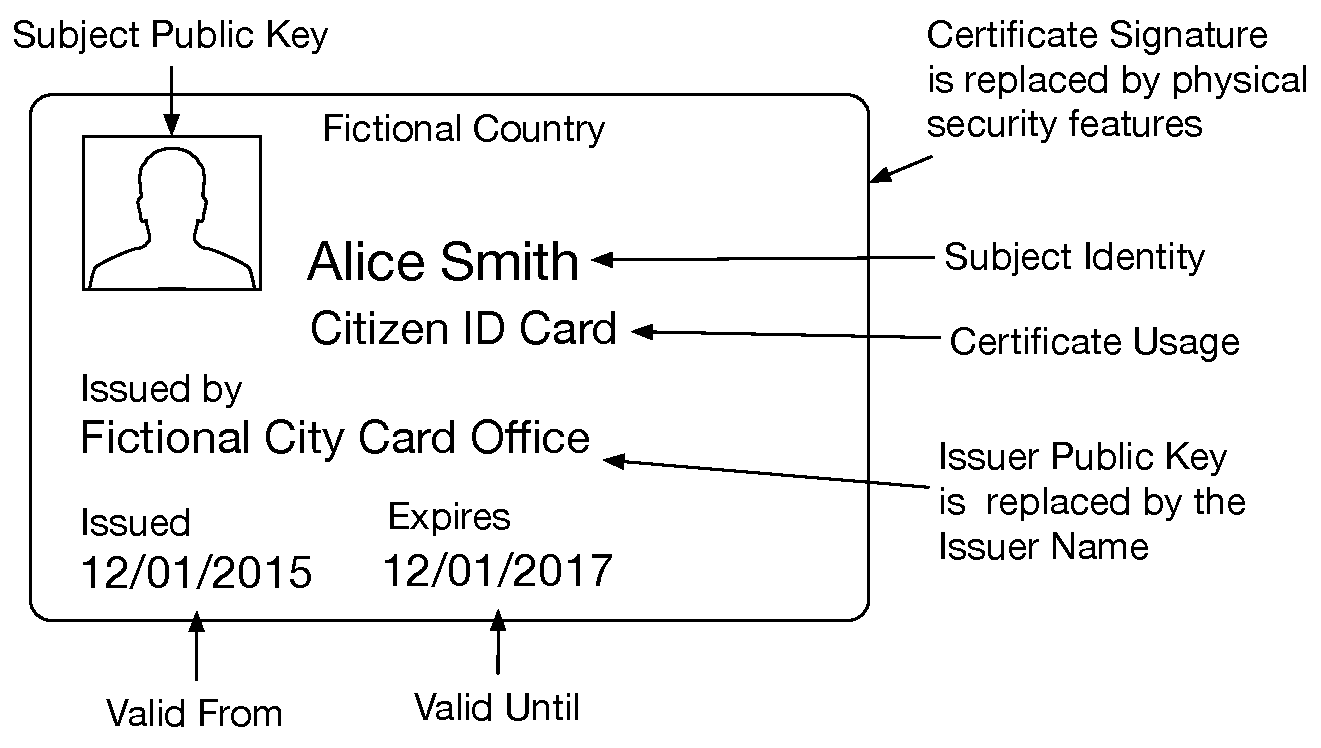
\includegraphics[width=85mm]{figures/id_card_as_certificate.pdf}
  \caption{
    An ID card is a certificate that binds a subject's full legal name
    (identity) to the subject's physical appearance, which acts as a public
    key.
  }
  \label{fig:id_card_as_certificate}
\end{figure}

Each government's ID card issuing operations are regulated by laws, so an ID
card's issue date can be used to track down the laws that make up its
certification policy. Last, the security of ID cards does not (yet) rely on
cryptographic primitives. Instead, ID cards include physical security measures
designed to deter tampering and prevent counterfeiting .


\subsubsection{Key Agreement Protocols}
\label{sec:key_agreement}

The initial design of symmetric key primitives, introduced in
\S~\ref{sec:crypto_primitives}, assumed that when two parties wish to interact,
one party generates a secret key and shares it with the other party using a
communication channel with privacy and integrity guarantees. In practice, a
pre-existing secure communication channel is rarely available.

\textit{Key agreement protocols} are used by two parties to establish a shared
secret key, and only require a communication channel with integrity guarantees.
Figure~\ref{fig:dh_key_exchange} outlines the Diffie-Hellman Key
Exchange~(DKE)~\cite{diffie1976keyexchange} protocol, which should give the
reader an intuition for how key agreement protocols work.

\begin{figure}[hbt]
  \centering
  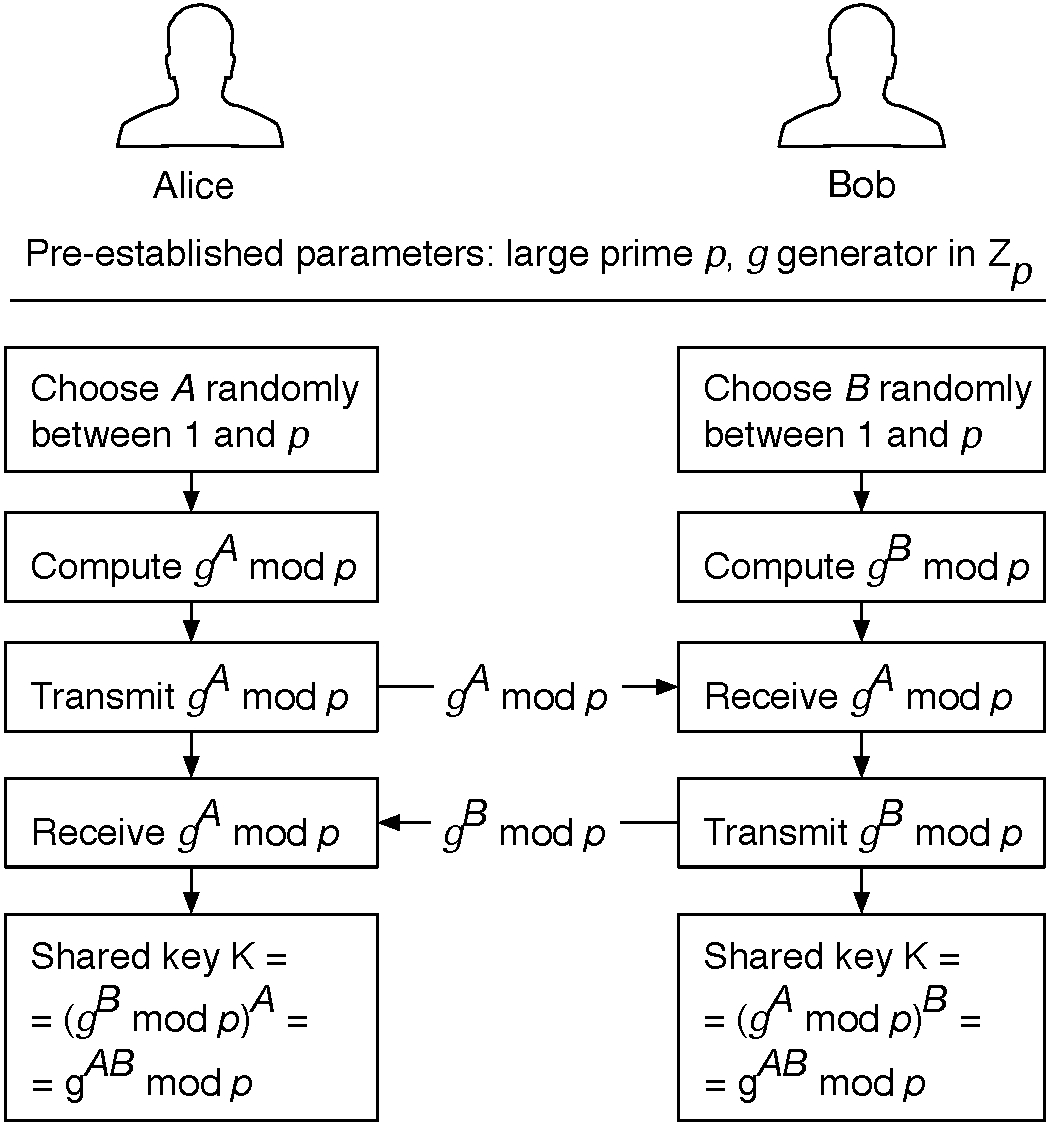
\includegraphics[width=80mm]{figures/dh_key_exchange.pdf}
  \caption{
    In the Diffie-Hellman Key Exchange (DKE) protocol, Alice and Bob
    agree on a shared secret key $K = g^{AB} \mod p$. An adversary that
    observes $g^{A} \mod p$ and $g^{B} \mod p$ cannot compute $K$.
  }
  \label{fig:dh_key_exchange}
\end{figure}

This work is interested in using key agreement protocols to build larger
systems, so we will neither explain the mathematic details in DKE, nor prove
its correctness. We note that both Alice and Bob derive the same shared secret
key, $K = g^{AB} \mod p$, without ever transmitting $K$. Furthermore, the
messages transmitted in DKE, namely $g^{A} \mod p$ and $g^{B} \mod p$, are not
sufficient for an eavesdropper Eve to determine $K$, because efficiently
solving for $x$ in $g^{x} \mod p$ is an open problem assumed to be very
difficult.

Key agreement protocols require a communication channel with integrity
guarantees. If an active adversary Eve can tamper with the messages transmitted
by Alice and Bob, she can perform a \textit{man-in-the-middle} (MITM) attack,
as illustrated in Figure~\ref{fig:key_agreement_mitm}.

\begin{figure}[hbt]
  \centering
  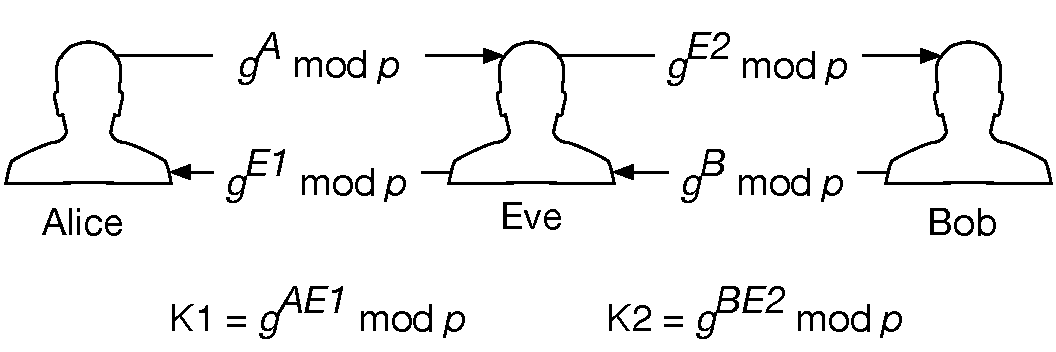
\includegraphics[width=85mm]{figures/key_agreement_mitm.pdf}
  \caption{
    Any key agreement protocol is vulnerable to a man-in-the-middle (MITM)
    attack. The active attacker performs key agreements and establishes shared
    secrets with both parties. The attacker can then forward messages between
    the victims, in order to observe their communication. The attacker can also
    send its own messages to either, impersonating the other victim.
  }
  \label{fig:key_agreement_mitm}
\end{figure}

In a MITM attack, Eve intercepts Alice's first key exchange message, and sends
Bob her own message. Eve then intercepts Bob's response and replaces it with
her own, which she sends to Alice. Eve effectively performs key exchanges with
both Alice and Bob, establishing a shared secret with each of them, without
either Bob or Alice being aware of her presence.

After establishing shared keys with both Alice and Bob, Eve can choose to
observe the communication between Alice and Bob, by forwarding messages between
them. For example, when Alice transmits a message, Eve can decrypt it using K1,
the shared key between herself and Alice. Eve can then encrypt the message with
K2, the key established between Bob and herself. While Bob still receives
Alice's message, Eve has been able to see its contents.

Furthermore, Eve can impersonate either party in the communication. For
example, Eve can create a message, encrypt it with K2, and then send it to Bob.
As Bob thinks that K2 is a shared secret key established between himself and
Alice, he will believe that Eve's message comes from Alice.

MITM attacks on key agreement protocols can be foiled by authenticating the
party who sends the last message in the protocol (in our examples, Bob) and
having it sign the key agreement messages. When a CA system is in place, Bob
uses his public key to sign the messages in the key agreement and also sends
Alice his certificate, along with the certificates for any intermediate CAs.
Alice validates Bob's certificate, ensures that the subject identified by the
certificate is who she expects (Bob), and verifies that the key agreement
messages exchanged between her and Bob match the signature provided by Bob.

In conclusion, a key agreement protocol can be used to bootstrap symmetric key
primitives from an asymmetric key signing scheme, where only one party needs to
be able to sign messages.


%\subsubsection{Cryptography for Storage}

\section{Security Model}
\label{sec:attestation}

THe central context of SGX is the \textit{enclave}, a protected environment
that contains the code and data pertaining to a security-sensitive computation.
An SGX-enabled processor protects the integrity and privacy of the computation
inside an enclave by isolating the enclave's code and data from the outside
environment, including the operating system and hypervisor, and hardware
devices attached to the system bus. At the same time, the SGX model remains
compatible with the the traditional software layering in the Intel
architecture, where the OS kernel and hypervisor manage the computer's
resources. The rest of this section describes the security properties of
enclaves, discussing the trade-offs made while trying to balance security with
backwards compatibility.



Enclaves were designed to contain and protect the privacy-sensitive parts of an
application. All the code that handles private data must receive integrity
protection. Otherwise, a hostile environment could modify the code to leak
information about private data. Therefore, the SGX programming model prescribes
that code which accesses private data must be entirely contained inside an
enclave. Jumping into and out of enclave code must be performed explicitly
using the dedicated instructions \texttt{EENTER} and \texttt{EEXIT}.

The code inside an enclave runs at ring 3 (user mode), so it has the same
privileges as regular application code (see Figure \ref{fig:cpu_rings}).

\begin{figure}[hbtp]
  \center{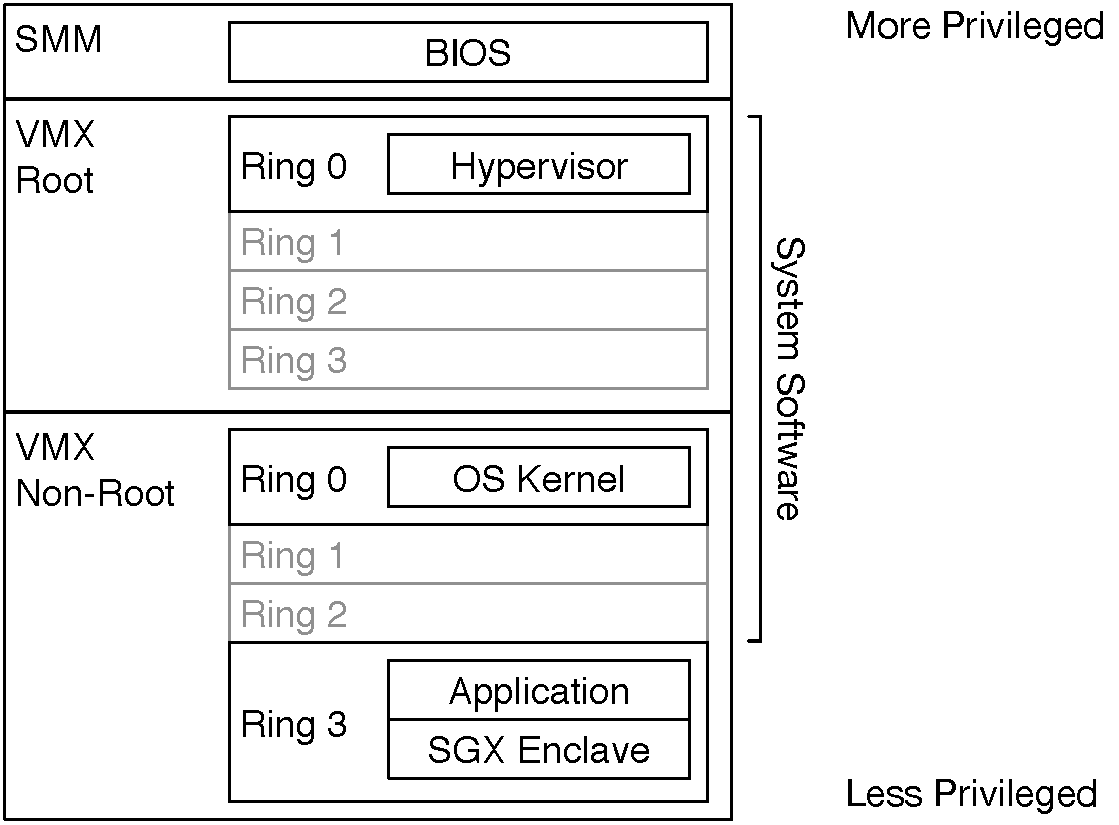
\includegraphics[width=75mm]{figures/cpu_rings.pdf}}
  \caption{
    Enclaves hold an application's private data and the code that operates on
    it. Therefore, they run at ring 3, in user mode.
  }
  \label{fig:computing_model}
\end{figure}

\subsection{Physical Attacks}
\label{sec:physical_attacks}

Physical attacks are generally classified according to their cost, which
factors in the equipment needed to carry out the attack and the attack's
complexity. Joe Grand's DefCon presentation~\cite{grand2004physicalattacks}
provides a good overview with a large number of intuition-building pictures.

The simplest type of physical attack is a denial of service attack performed by
disconnecting the victim computer's power supply or network cable. The threat
models of most secure architectures ignore this attack, because denial of
service can also be achieved by software attacks that compromise the computer's
system software, such as the hypervisor.


\subsubsection{Port Attacks}
\label{sec:physical_port_attacks}

Slightly more involved attacks rely on connecting a device to an existing port
on the victim computer's case or motherboard~(\S~\ref{sec:motherboard}). A
simple example is a \textit{cold boot attack}, where the attacker plugs in a
USB flash drive into the victim's case and causes the computer to boot from
the flash drive, whose malicious system software receives unrestricted access
to the computer's peripherals.

More expensive physical attacks that still require relatively little effort
target the debug ports of various peripherals. The cost of these attacks is
generally dominated by the expense of acquiring the development kits needed to
connect to the debug ports. For example, recent Intel processors include the
Generic Debug eXternal Connection~(GDXC)~\cite{yuffe2011sandybridge,
intel2011gdxc}, which collects and filters the data transfered by the uncore's
ring bus (\S~\ref{sec:cache_coherence}), and reports it to an external
debugger.

The threat models of secure architectures generally ignore debug port attacks,
under the assumption that devices sold for general consumption have their debug
ports irreversibly disabled. In practice, manufacturers have strong incentives
to preserve debugging ports in production hardware, as this facilitates the
diagnosis and repair of defective units. Due to insufficient documentation on
this topic, we ignore the possibility of GDXC-based attacks. Fortunately, a
recent Intel patent~\cite{shanbhogue2015gdxcsgx} indicates that Intel engineers
are tackling at least some classes of attacks targeting debugging ports.


\subsubsection{Bus Tapping Attacks}
\label{sec:physical_bus_attacks}

More complex physical attacks consist of installing a device that taps a bus on
the computer's motherboard (\S~\ref{sec:motherboard}). \textit{Passive attacks}
are limited to monitoring the bus traffic, whereas \textit{active attacks} can
modify the traffic, or even place new commands on the bus. \textit{Replay
attacks} are a notoriously difficult to defeat class of active attacks, where
the attacker first records the bus traffic, and then selectively replays a
subset of the traffic. Replay attacks bypass systems that rely on static
signatures or HMACs, and generally aim to double-spend a limited resource.

The cost of bus tapping attacks is generally dominated by the cost of the
equipment used to tap the bus, which increases with bus speed and complexity.
For example, the flash chip that stores the computer's firmware is connected to
the PCH via an SPI bus (\S~\ref{sec:motherboard}), which is simpler and much
slower than the DDR bus connecting DRAM to the CPU. Consequently, tapping the
SPI bus is much cheaper than tapping the DDR bus. For this reason, systems
whose security relies on a cryptographiic hash of the firmware will first copy
the firmware into DRAM, hash the DRAM copy of the firmware, and then execute
the firmware from DRAM.

Although the DDR bus's speed makes tapping it very difficult, there are
well-publicized records of successful attempts. The original Xbox console's
booting process was reverse-engineered thanks to a passive tap on the DRAM
bus~\cite{huang2003xbox} that showed that the firmware used to boot the
console was partially stored in its southbridge. The protection mechanisms of
the PlayStation 3 hypervisor were subverted by an active tap on its memory
bus~\cite{hotz2010ps3} that targeted the hypervisor's page tables.

\S~\ref{sec:related} shows that concealing the addresses of the DRAM cells
accessed by a program is orders of magnitude more expensive than protecting the
memory's contents. Therefore, we are interested in analyzing attacks that tap
the DRAM bus, but only use the information on the address lines. These attacks
use the same equipment as normal DRAM bus tapping attacks, but require a
significantly more involved analysis to learn useful information. One of the
difficulties of such attacks is that the memory addresses observed on the DRAM
bus are generally very different from the application's memory access patterns,
because of the extensive cache hierachies in modern processors
(\S~\ref{sec:caching}).

We are not aware of any successful attack based on tapping the address lines of
a DRAM bus and analyzing the sequence of memory addresses.


\subsubsection{Chip Attacks}
\label{sec:physical_chip_attacks}

The most equipment-intensive physical attacks involve removing a chip's
packaging and directly interacting with its electrical circuits. These attacks
generally take advantage of equipment and techiques that were originally
developed to diagnose design and manufacturing defects in chips.
\cite{beck1998integrated} covers these techniques in depth.

The cost of chip attacks is dominated by the required equipment, although the
reverse-engineering involved is also non-trivial. This cost grows very rapidly
as the size of the circuitry's components decreases. At the time of this
writing, the latest Intel CPUs have a 14nm feature size, which requires ion
beam microscopy (TODO: look up the details for all this)

The least expensive class of chip attacks are destructive, and therefore only
require imaging the chip's circuitry. These attacks rely on a microscope
capable of capturing the necessary details in each layer, and equipment for
mechanically removing each layer and exposing the layer below it to the
microscope.

Imaging attacks generally target global secrets shared by all the chips in a
family, such as ROM masks that store global encryption keys or secret boot
code. They are also used to reverse-engineer undocumented functionality, such
as debugging backdoors. E-fuses and polyfuses are particularly vulnerable to
imaging attacks, because of their relatively large sizes.

Non-destructive passive chip attacks require measuring the voltages across a
module at specific times, while the chip is operating. These attacks are orders
of magnitude more expensive than imaging attacks, because the attacker must
maintain the integrity of the chip's circuitry, and therefore cannot de-layer
the chip.

The simplest active attacks on a chip consist in creating or destroying an
electric connection between two components. For example, the debugging
functionality in many chips is disabled by ``blowing'' an e-fuse. Once this
e-fuse is located, an attacker can reconnect its two ends, effectively undoing
the ``blowing'' operation. More expensive attacks involve changing voltages
across a component as the chip is operating, and are typically used to
reverse-engineer complex circuits.

Surprisingly, active attacks are not significantly more expensive to carry out
than passive non-destructive attacks. This is because the tools used to measure
the voltage across specific components are not very different from the tools
that can tamper with the chip's electric structure. Therefore, once an attacker
develops a process for accessing a module without destroying the chip's
circuitry, the attacker can use the same process for both passive and active
attacks.

At the architectural level, we cannot protect from physical attacks against the
CPU's chip package. Active attacks on the CPU change the computer's execution
semantics, leaving us without any hardware that can be trusted to make security
decisions. Passive attacks can read the private data that the CPU is
processing. Therefore, many secure computing architectures assume that the
processor chip package is invulnerable to physical attacks.

Thankfully, physical attacks can be deterred by reducing the value that an
attacker obtains by compromising an individual chip. As long as this value is
below the cost of carrying out the physical attack, a system's designer can
hope that the processor's chip package will not be targeted by the physical
attacks.

Architects can reduce the value of compromising an individual system by
avoiding shared secrets, such as global encryption keys. Chip designers can
increase the cost of a physical attack by not storing a platform's secrets in
hardware that is vulnerable to destructive attacks, such as e-fuses.


\subsubsection{Power Analysis Attacks}
\label{sec:power_analysis_attacks}

An entirely different approach to physical attacks consists of indirectly
measuring the power consumption of a computer system or its components. The
attacker takes advantage of a known correlation between power consumption and
the data being computed on, and learns some property of the data from the
observed power consumption.

The earliest power analysis attacks have directly measured the processor chip's
power consumption. For example, [] used the correlation between the power
consumed by a smart card chip's multiplication circuitry and the number of one
bits in the input, and learned an RSA key that the smart card was supposed to
safeguard.

While direct power analysis attacks necessitate some equipment, their costs are
dominated by the complexity of the analysis required to learn the desired
information from the observed power trace which, in turn, is determined by the
complexity of the processor's circuitry. Today's smart cards contain special
circuitry designed to frustrate power analysis attacks. [] We are not aware of
any successful power analysis attacks against full-blown out-of-order Intel
processors.

Unfortunately, power analysis attacks can be extended to displays and human
input devices, which cannot be secured in any reasonable manner. For example,
[] measured the radiation emitted by a CRT display's ion beam to reconstitute
the image on a computer screen in a different room. [] used a directional
microphone to measure the sound emitted by a keyboard and learn the password
that its operator typed. [] applied similar techniques to learn a user's input
on a smartphone's on-screen keyboard, based on data from the device's
accelerometer.

In general, power attacks cannot be addressed at the architectural level, as
they rely on implementation details that are decided during the manufacturing
process. Therefore, it is unsurprising that the secure computing architectures
described in \S~\ref{sec:related} do not protect against power analysis
attacks.

\subsection{Privileged Software Attacks}
\label{sec:system_software_attacks}

The rest of this section points to successful exploits that execute at each of
the privilege levels described in \S~\ref{sec:rings}, motivating the SGX design
decision to assume that all the privileged software on the computer is
malicious. \cite{rutkowska2015intelsux} describes all the programmable hardware
inside Intel computers, and outlines the security implications of compromising
the software running it.

SMM, the most privileged execution level, is only used to handle a specific
kind of interrupts (\S~\ref{sec:interrupts}), namely
\textit{System Management Interrupts} (SMI). SMIs were initially designed
exclusively for hardware use, and were only triggered by asserting a dedicated
pin (SMI\#) in the CPU's chip package. However, in modern systems, system
software can generate an SMI by using the LAPIC's IPI mechanism. This opens up
the avenue for SMM-based software exploits.

The SMM handler is stored in  \textit{System Management RAM} (SMRAM) which, in
theory, is not accessible when the processor isn't running in SMM. However, its
protection mechanisms were bypassed multiple times~\cite{duflot2006smm,
rutkowska2008remap, wojtczuk2009smm, kallenberg2014smm}, and SMM-based
rootkits~\cite{wecherowski2009smm, embleton2010smm} have been demonstrated.
Compromising the SMM grants an attacker access to all the software on the
computer, as SMM is the most privileged execution mode.

Xen \cite{zhang2008xen} is a very popular representative of the family of
hypervisors that run in VMX root mode and use hardware virtualization. At
150,000 lines of code~\cite{xen2015loc}, Xen's codebase is relatively small,
especially when compared to a kernel. However, Xen still has had over 40
security vulnerabilities patched in \textbf{each} of the last three years
(2012-2014) \cite{cvedetails2014xen}.

\cite{mccune2010trustvisor} proposes using a very small hypervisor together
with Intel TXT's dynamic root of trust for measurement (DRTM) to implement
trusted execution. \cite{vasudevan2010requirements} argues that a dynamic root
of trust mechanism, like Intel TXT, is necessary to ensure a hypervisor's
integrity.  Unfortunately, the TXT design requires an implementation complex
enough that exploitable security vulnerabilities have creeped in
\cite{wojtczuk2009txt2, wojtczuk2011txt}. Furthermore, any SMM attack can be
used to compromise TXT \cite{wojtczuk2009txt}.

The monolithic kernel design leads to many opportunities for security
vulnerabilities in kernel code. Linux is by far the most popular kernel for
IaaS cloud environments. Linux has \emph{17 million} lines of
code~\cite{anthony2014linuxsize}, and  has had over 100 security
vulnerabilities patched in \textbf{each} of the last three years
(2012-2014)~\cite{cvedetails2014linux, chen2011linux}.

\subsection{Software Attacks on Peripherals}
\label{sec:device_attacks}

Threat models for secure architectures generally only consider software attacks
that directly target other components in the software stack running on the CPU.
This assumption results in security arguments with the very desirable property
of not depending on implementation details, such as the structure of the
motherboard hosting the processor chip.

The threat models mentioned above must classify attacks from other motherboard
components as physical attacks. Unfortunately, these models would mis-classify
all the attacks described in this sub-section, which can be carried out solely
by executing software on the victim processor. The incorrect classification
matters in cloud computing scenarios, where physical attacks are significantly
more expensive than software attacks.

The PCIe bus~(\S~\ref{sec:motherboard}) allows any device connected to the bus
to perform \textit{Direct Memory Access}~(DMA), reading from and writing to
the computer's DRAM without the involvement of a CPU core. Each device is
assigned a DRAM range via a standard PCI configuration mechanism, but the bus
does not restrict a device from performing DMA targeting DRAM outside its
assigned range.

Without any additonal protection mechanism, an attacker that compromises system
software can take advantage of programmable devices to access any DRAM region,
yielding capabilities that were traditionally associated with a DRAM bus tap.
For example, an early implementation of Intel TXT~\cite{grawrock2009txt} was
compromised by programming a PCIe NIC to read TXT-reserved DRAM via DMA
transfers~\cite{wojtczuk2011txt}. Recent versions have addressed this attack by
adding extra security checks in the DMA bus arbiter. \S~\ref{sec:intel_txt}
provides a more detailed description of Intel TXT.

The rowhammer DRAM bit-flipping attack~\cite{kim2014rowhammer,
google2015rowhammer, gruss2015rowhammer} is an example of a different class of
software attacks that exploit design defects in the computer's hardware.
Rowhammer took advantage of the fact that some mobile DRAM
chips~(\S~\ref{sec:motherboard}) refreshed the DRAM's contents slowly enough
that repeatedly changing the contents of a memory cell could impact the charge
stored in a neighboring cell, which resulted in changing the bit value obtained
from reading the cell. By carefully targeting specific memory addresses, the
attackers caused bit flips in the page tables used by the CPU's address
translation (\S~\ref{sec:paging}) mechanism, and in other data structures used
to make security decisions.

The issue exploited by the rowhammer attack most likely stems from an incorrect
design assumption. The DRAM engineers probably only thought of non-malicious
software and assumed that an individual DRAM cell cannot be accessed too
often, as repeated accesses to the same memory address would be absorbed by the
CPU's caches (\S~\ref{sec:caching}). However, malicious software can take
advantage of the \texttt{CLFLUSH} instruction, which flushes the cache line
that contains a given DRAM address. \texttt{CLFLUSH} is intended as a method
for applications to extract more performance out of the cache hierarchy, and
is therefore available to software running at all privilege levels. Rowhammer
exploited the interaction between \texttt{CLFLUSH}'s availability and the DRAM
engineers' invalid assumptions to obtain capabilities that are normally
associated with an active DRAM bus attack.

% On Die Digital Thermal Sensors: SDM S 14.7.5

Intel's \textit{Software Development Manual}~(SDM)~\cite{intel2015sdm} and
Optimization Reference Manual~\cite{intel2014optimization} describe a vast
array of performance monitoring events exposed by recent Intel processors,
such as branch mispredictions (\S~\ref{sec:out_of_order}). The SDM also
describes digital temperature sensors embedded in each CPU core, whose readings
are exposed using Model-Specific Registers~(MSRs)~(\S~\ref{sec:address_spaces})
that can be read by system software.

An attacker that compromises a computer's system software and gains access to
the performance monitoring events or the temperature sensors can obtain the
information needed to carry out a power analysis attack, which normally
requires physical access to the victim computer and specialized equipment.

Virtually all motherboards store the firmware used to boot the computer in a
flash memory chip (\S~\ref{sec:motherboard}) that can be written by system
software. This implementation strategy provides an inexpensive avenue for
deploying firmware bug fixes. At the same time, an attack that compromises the
system software can subvert the firmware update mechanism to inject malicious
code into the firmware. The malicious code can be used to carry out a cold boot
attack, which is typically considered a physical attack. Furthermore, malicious
firmware can run code at in System Management Mode (SMM, \S~\ref{sec:rings}),
the highest software privilege level. Last, malicious firmware can modify the
system software as it is loaded during the boot process. These avenues give the
attacker capabilities that have traditionally been associated with DRAM bus
tapping attacks.

The Intel Management Engine (ME)~\cite{ruan2014intelme} loads its firmware
from the same flash memory chip as the main computer, which opens up the
possibility of compromising its firmware. Due to its vast management
capabilities (\S~\ref{sec:intel_me}), a compromised ME would bring most of the
powers that come with installing active probes on the DRAM bus, the PCI bus,
and the System Management bus (SMBus), as well as power consumption meters.
Thanks to its direct access to the motherboard's Ethernet PHY, the probe would
be able to communicate with the attacker while the computer is in the Soft-Off
state, also known as S5, where the computer is mostly powered off, but is still
connected to a power source.  The ME has significantly less computational power
than probe equipment, however, as it uses low-power embedded components, such
as a 200-400Mhz execution core, and about 600KB of internal RAM.

The computer and ME firmware are protected by a few security measures. The
first line of defense is a security check in the firmware's update sevice,
which only accepts firmware updates that have been digitally signed by a
manufacturer key that is hard-coded in the firmware. This protection can be
circumvented with relative ease by foregoing the firmware's update services,
and instead accessing the flash memory chip directly, via the PCH's SPI bus
controller.

The deeper, more powerful, lines of defense against firmware attacks are rooted
in the CPU and ME's hardware. The bootloader in the ME's ROM will only load
flash firmware that contains a correct signature generated by a specific Intel
RSA key. The ME's boot ROM contains the SHA-256 cryptographic hash of the RSA
public key, and uses it to validate the full Intel public key stored in the
signature. Similarly, the microcode bootstrap process in recent CPUs will only
execute firmware in an Authenticated Code Module
(ACM, \S~\ref{sec:uefi_sec_details}) signed by an Intel key whose SHA-256 hash
is hard-coded in the microcode ROM.

However, both the computer firmware security checks \cite{wojtczuk2010bios,
furtak2014bios} and the ME security checks \cite{tereshkin2009amt} have been
subverted in the past. While the approaches described above are theoretically
sound, the intricate details and complex interactions in Intel-based systems
make it very likely that security vulnerabilities will creep into
implementations. Further proving this point, a security
analysis~\cite{ververis2010security} found that early versions of Intel's
Active Management Technology~(AMT), the flagship ME application, contained an
assortment of security issues that allowed an attacker to completely take over
a computer whose ME firmware contained the AMT application.

The attacks described in this section show that a system whose threat model
assumes no software attacks must be designed with an understanding of all the
system's buses, the programmable devices that may be attached to them. The
system's security analysis must argue that the devices will not be used in
physical-like attacks. The argument will rely on barriers that prevent
untrusted software running on the CPU from communicating with other
programmable devices, and on barriers that prevent compromised programmable
devices from tampering with sensitive buses or DRAM.

Unfortunately, the ME, PCH and DMI are Intel-proprietary and largely
undocumented, so we cannot assess the security of the measures set in place to
protect the ME from being compromised, and we cannot reason about the impact
of a compromised ME that runs malicious software.

\subsection{Address Translation Attacks}
\label{sec:paging_attacks}

\S~\ref{sec:system_software_attacks} argues that today's system software is
virtually guaranteed to have security vulnerabilities. This suggests that a
cautious secure architecture shoild avoid having the system software in the
TCB.

However, removing the system software from the TCB requires that the
architecture provides a method for isolating sensitive application code from
the untrusted system software. This is typically accomplished by a designing a
mechanism for loading application code in isolated containers whose contents
can be certified via software
attestation~(\S~\ref{sec:generic_software_attestation}). One of the more
difficult problems faced by these designes is that application software relies
on the memory management services provided by the system software, which is now
untrusted.

Intel's SGX~\cite{mckeen2013sgx, anati2013sgx}, which was inspired by
Bastion~\cite{champagne2010bastion}, leaves the system software in charge of
setting up the page tables (\S~\ref{sec:paging}) used by address translation,
but instates access checks that prevent the system software from directly
accessing the isolated container's memory.

This section discusses some attacks that become relevant when the application
software does not trust the system software which in charge of the page tables.
Understanding these attacks is a prerequisite to reasoning about the security
properties of architectures with this threat model. For example, a large amount
of the mechanisms in SGX are aimed at dealing with a subset of the attacks
described here.


\subsubsection{Passive Attacks}
\label{sec:fault_tracking_attacks}

System software uses the the CPU's address translation feature
(\S~\ref{sec:paging}) to implement page swapping, where infrequently used
memory pages are evicted from DRAM to a slower storage medium. Page swapping
relies the accessed (A) and dirty (D) page table entry attributes
(\S~\ref{sec:page_table_attributes}) to identify the DRAM pages to be evicted,
and on a page fault handler (\S~\ref{sec:faults}) to bring evicted pages back
into DRAM when they are accessed.

Unfortunately, the features that support efficient page swapping turn into a
security liability, when the system software managing the page tables is not
trusted by the application software using the page tables. The system software
can be prevented from reading the application's memory directly by placing the
application in an isolated container. However, potentially malicious system
software can still infer partial information about the application's memory
access patterns, by observing the application's page faults and page table
attributes.

We consider this class of attacks to be passive attacks that exploit the CPU's
address translation feature. It may seem that the page-level memory access
patterns provided by these attacks are not very useful. However,
\cite{xu2015pagefaults} describes how this attack can be carried out against
Intel's SGX, and implements the attack in a few practical settings. In one
scenario, which is particularly concerning for medical image processing,
the outline of a JPEG image is inferred while the image is decompressed inside
a container protected by SGX's isolation guarantees.


\subsubsection{Active Attacks}
\label{sec:memory_mapping_attacks}

We define active address translation attacks to be the class of attacks where
malicious system software modifies the page tables used by an application in
a way that breaks the virtual memory abstraction (\S~\ref{sec:paging}). Memory
mapping attacks do not include scenarios where the system software breaks the
memory abstraction by directly writing to the application's memory pages.

We begin with an example of a straight-forward active attack. In this example,
the application inside a protected container performs a security check to
decide whether to disclose some sensitive information. Depending on the
security check's outcome, the enclave code either calls a \texttt{errorOut}
procedure, or a \texttt{disclose} procedure. The simplest vesion of the attack
assumes that each procedure's code starts at a page boundary, and takes up less
than a page. These assumptions are relaxed in more complex versions of the
attack.

In the most straight-forward setting, the malicious system software directly
modifies the page tables of the application inside the container, as shown in
Figure~\ref{fig:active_mapping_attack}, so the virtual address intended to
store the \texttt{errorOut} procedure is actually mapped to a DRAM page that
contains the \texttt{disclose} procedure. Without any security measures in
place, when the application's code jumps to the virtual address of the
\texttt{errorOut} procedure, the CPU will execute the code of the
\texttt{disclose} procedure instead.

\begin{figure}[hbt]
  \centering
  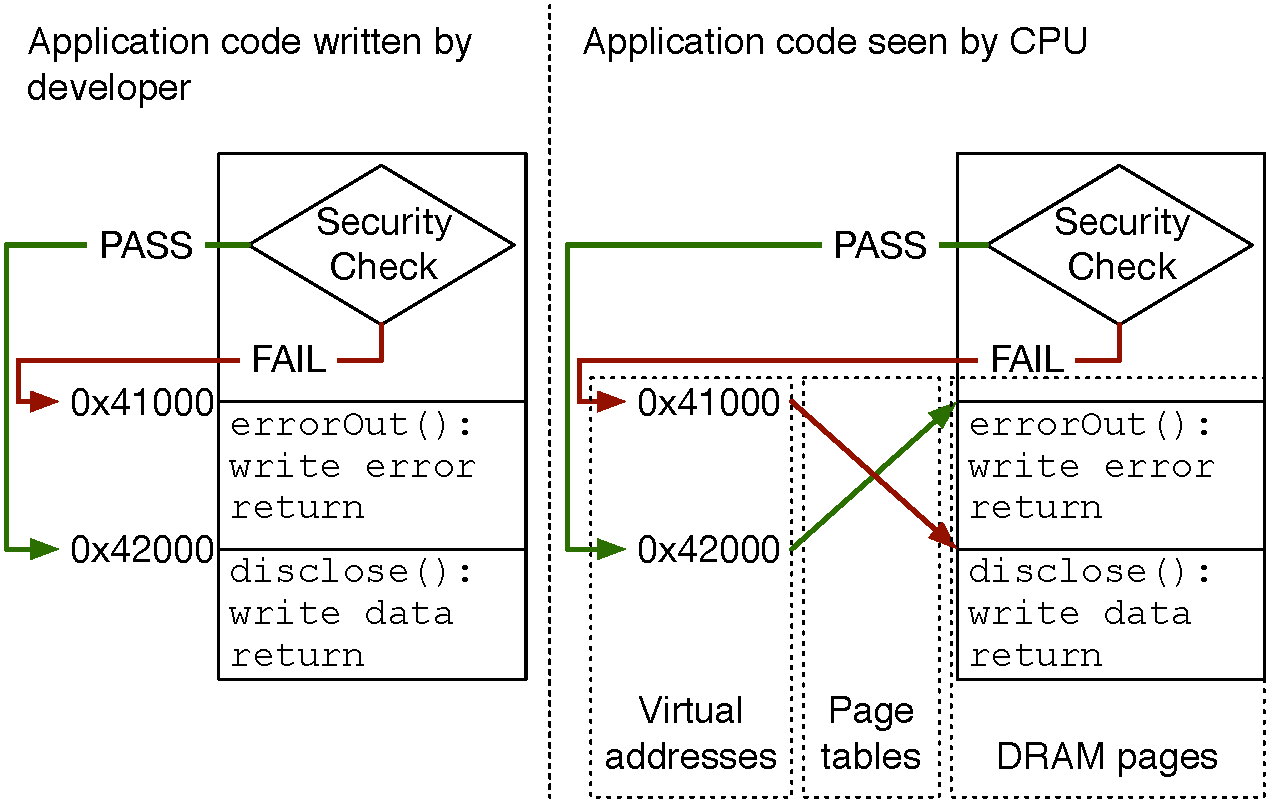
\includegraphics[width=85mm]{figures/active_mapping_attack.pdf}
  \caption{
    An example of an active memory mapping attack. The application's author
    intends to peform a security check, and only disclose a piece of sensitive
    information if the check passes. Malicious system software maps the virtual
    address of the procedure called when the security check fails to a DRAM
    page that contains the procedure that discloses the sensitive information,
    which is supposed to be called when the security check passes.
  }
  \label{fig:active_mapping_attack}
\end{figure}

The most obvious active attacks on memory mapping can be defeated by tracking
the correct virtual address for each DRAM page that belongs to a protected
container. However, a naive protection measure based on address tracking can be
defeated by a more subtle active attack that relies on the architectural
support for page swapping. Figure~\ref{fig:swap_mapping_attack} illustrates an
attack that does not modify the application's page tables, but produces the
same corrputed CPU view of the application as the straight-forward attack
described above.

\begin{figure}[hbt]
  \centering
  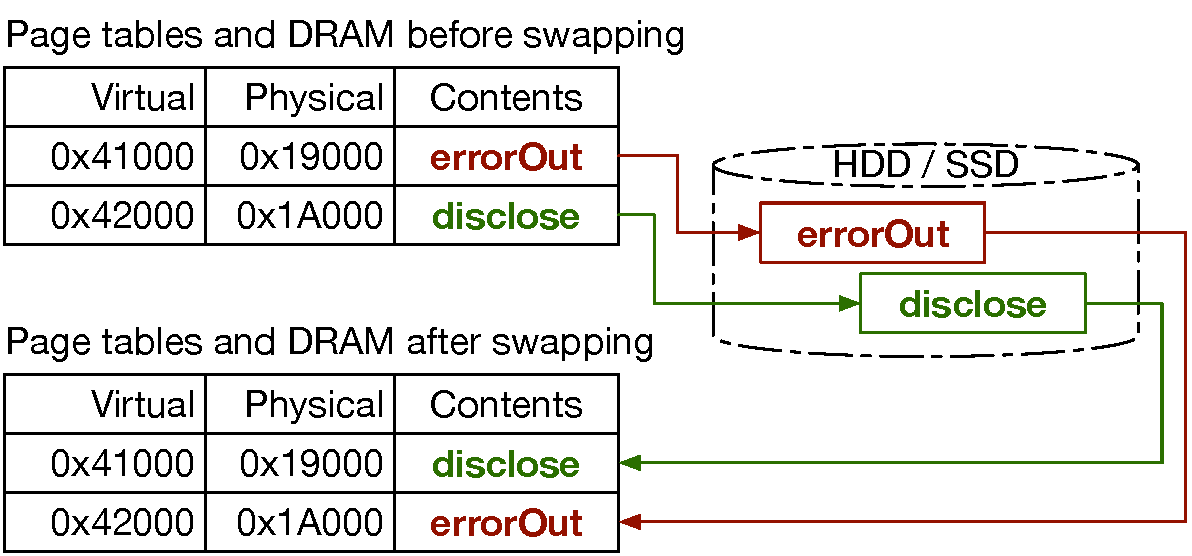
\includegraphics[width=85mm]{figures/swap_mapping_attack.pdf}
  \caption{
    An active memory mapping attack where the system software does not modify
    the page tables. Instead, two pages are evicted from DRAM to a slower
    storage medium. The malicious system software swaps the two pages' contents
    then brings them back into DRAM, building the same incorrect page mapping
    as the direct attack shown in Figure~\ref{fig:active_mapping_attack}. This
    attack defeats protection measures that rely on tracking the virtual and
    disk addresses for DRAM pages.
  }
  \label{fig:swap_mapping_attack}
\end{figure}

In the swapping attack, malicious system software evicts the pages that contain
the \texttt{errorOut} and \texttt{disclose} procedures from DRAM to a slower
medium, such as a hard disk. The system software exchanges the hard disk
bytes storing the two pages, and then brings the two pages back into DRAM.
Remarkably, all the steps taken by this attack are indistinguishable from
legitimate page swapping activity, with the exception of the I/O operations
that exchange the disk bytes that store evicted pages.

The subtle attack described above can be defeated by cryptographically
binding the contents of each page that is evicted from DRAM to the virtual
address that the page should be mapped to. The cryptographic primitive
(\S~\ref{sec:crypto_primitives}) used to perform the binding must obiously
guarantee integrity. Furthermore, it must also guarantee freshness, in order
to foil replay attacks where the system software ``undoes'' an application's
writes by evicting one of its DRAM pages to disk and bringing in an older
version of the same page.

Today's multi-core architectures can be subjected to an even more subtle active
attack, illustrated in Figure~\ref{fig:tlb_mapping_attack}, which can bypass
any protection measures that solely focus on the integrity of the page tables.

\begin{figure}[hbt]
  \centering
  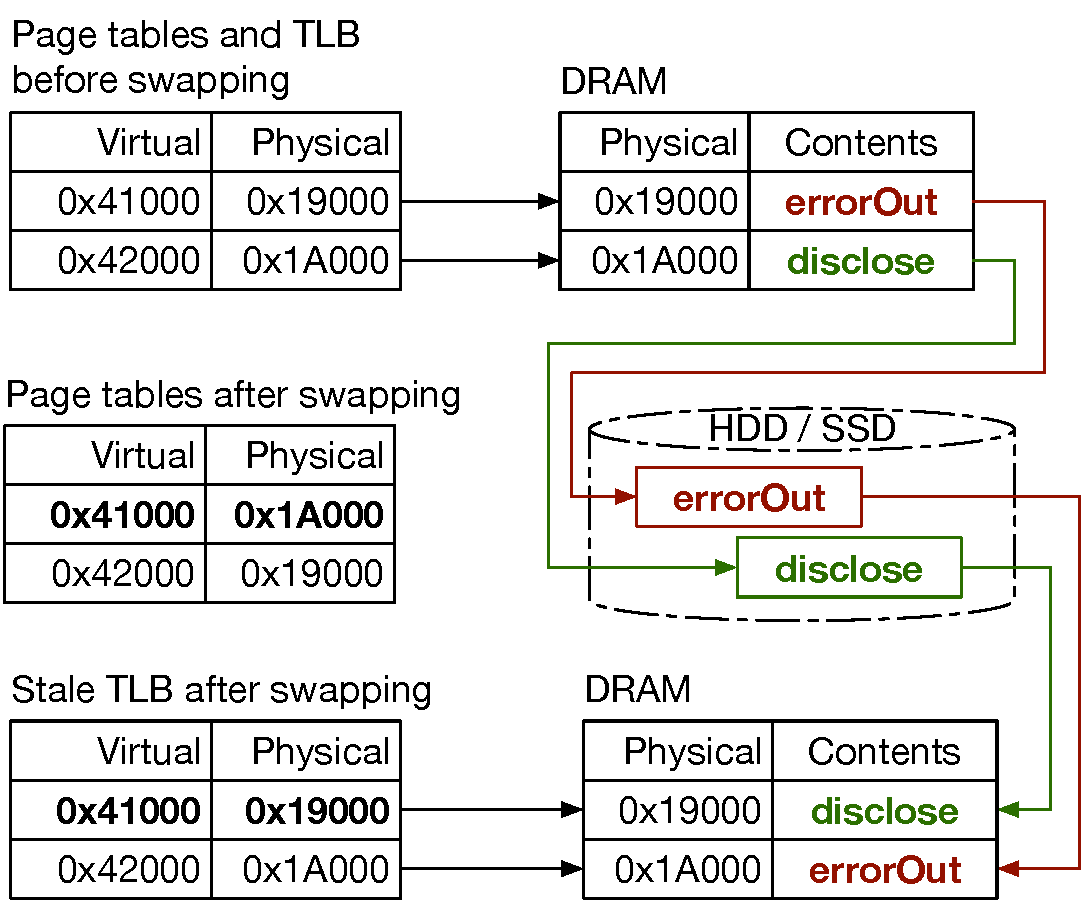
\includegraphics[width=75mm]{figures/tlb_mapping_attack.pdf}
  \caption{
    An active memory mapping attack where the system software does not
    invalidate a core's TLBs when it evicts two pages from DRAM and exchanges
    their locations when reading them back in. The page tables are updated
    correctly, but the core with stale TLB entries has the same incorrect view
    of the protected container's code as in
    Figure~\ref{fig:active_mapping_attack}.
  }
  \label{fig:tlb_mapping_attack}
\end{figure}

For performance reasons, each execution core caches address translation results
in its own translation look-aside buffer~(TLB,~\S~\ref{sec:tlbs}). For
simplicity, the TLBs are not covered by the cache coherence protocol that
synchronizes data caches across cores. Instead, the system software is
responsible for invalidating TLB entries across all the cores when it modifies
the page tables.

Malicious system software can take advantage of the design decisions explained
above by carring out the following attack. While the same software used in the
previous examples is executing on a core, the system software executes on a
different core and evicts the \texttt{errorOut} and \texttt{disclose} pages
from DRAM. Like in the previous attack, the system software loads the
\texttt{disclose} code in the DRAM page that previously held \texttt{errorOut}.
In this attack, however, the system software also updates the page tables.

The core where the system software executed sees the code that the application
developer intended. Therefore, the attack will pass any security checks that
rely cryptographic associations between page contents and page table data, as
long as the checks are performed by the core used to load pages back into DRAM.
However, the core that executes the protected container's code still uses the
old page table data, because the system software did not invalidate its TLB
entries. Assuming the TLBs are not subjected to any additional security checks,
this attack causes the same private information leak as the previous examples.

In order to avoid the last attack described in this section, the trusted
software or hardware that implements protected containers must also ensure that
the system software invalidates the relevant TLB entries on all the cores when
it evicts a page from a protected container to DRAM.

\HeadingLevelB{Cache Timing Attacks}
\label{sec:cache_timing}

Cache timing attacks~\cite{banescu2011cache} are a powerful class of software
attacks that can be mounted entirely by application code running at ring 3
(\S~\ref{sec:rings}). Cache timing attacks do not learn information by reading
the victim's memory, so they bypass the address translation-based isolation
measures (\S~\ref{sec:paging}) implemented in today's kernels and hypervisors.


\HeadingLevelC{Theory}

Cache timing attacks exploit the unfortunate dependency between the location of
a memory access and the time it takes to perform the access. A cache miss
requires at least one memory access to the next level cache, and might require
a second memory access if a write-back occurs. On the Intel architecture, the
latency between a cache hit and a miss can be easily measured by the
\texttt{RDTSC} and \texttt{RDTSCP} instructions (\S~\ref{sec:address_spaces}),
which read a high-resolution time-stamp counter. These instructions have been
designed for benchmarking and optimizing software, so they are available to
ring 3 software.

The fundamental tool of a cache timing attack is an attacker process that
measures the latency of accesses to carefully designated memory locations in
its own address space. The memory locations are chosen so that they map to
the same cache lines as some interesting memory locations in a victim process,
in a cache that is shared between the attacker and the victim. This requires
in-depth knowledge of the shared cache's organization (\S~\ref{sec:cache_org}).

Armed with the knowledge of the cache's organization, the attacker process
sets up the attack by accessing its own memory in such a way that it fills up
all the ways in the cache sets that would hold the victim's interesting memory
locations. After the targeted cache sets are full, the attacker allows the
victim process to execute. When the victim process accesses an interesting
memory locations in its own address space, the shared cache must evict one of
the cache lines holding the attacker's memory locations.

As the victim is executing, the attacker process repeatedly times accesses to
its own memory locations. When the access times indicate that a location was
evicted from the cache, the attacker can conclude that the victim accessed an
interesting memory location in its own cache. Over time, the attacker collects
the results of many measurements and learns a subset of the victim's memory
access pattern. If the victim processes sensitive information using
data-dependent memory fetches, the attacker may be able to deduce the sensitive
information from the learned memory access pattern.


\HeadingLevelC{Practical Considerations}

Cache timing attacks require control over a software process that shares a
cache memory with the victim process. Therefore, a cache timing attack that
aims at the L2 cache would have to rely on the system software to schedule a
software thread on a logical processor in the same core as the target software,
whereas an attack on the L3 cache can be performed using any logical processor
on the same CPU. The latter attacks rely on the fact that the L3 cache is
inclusive, which greatly simplifies the processor's cache coherence
implementation (\S~\ref{sec:cache_coherence}).

The cache sharing requirement implies that L3 cache attacks are feasible in an
IaaS environment, whereas L2 cache attacks become a significant concern when
running sensitive software on a user's desktop.

Out-of-order execution (\S~\ref{sec:out_of_order}) can introduce noise in cache
timing attacks. First, memory accesses may not be performed in program order,
which can impact the lines selected by the cache eviction algorithms. Second,
out-of-order execution may result in cache fills that do not correspond to
executed instructions. For example, a load that follows a faulting instruction
may be scheduled and executed before the fault is detected.

Cache timing attacks must account for speculative execution, as mispredicted
memory accesses can still cause cache fills. Therefore, the attacker may
observe cache fills that don't correspond to instructions that were actually
executed by the victim software. Memory prefetching adds further noise to cache
timing attacks, as the attacker may observe cache fills that don't correspond
to instructions in the victim code, even when accounting for speculative
execution.


\HeadingLevelC{Known Cache Timing Attacks}

Despite these difficulties, cache timing attacks are known to retrieve
cryptographic keys used by AES~\cite{osvik2006aes, bonneau2006aes},
RSA~\cite{brumley2005rsa}, Diffie-Hellman~\cite{kocher1996timing}, and
elliptic-curve cryptography~\cite{brumley2011ecc}.

Early attacks required access to the victim's CPU core, but more sophisticated
recent attacks~\cite{yarom2013llctiming, liu2015llctiming} are able to use the
L3 cache, which is shared by all the cores on a CPU die. L3-based attacks can
be particularly devastating in cloud computing scenarios, where running
software on the same computer as a victim application only requires modest
statistical analysis skills and a small amount of
money~\cite{ristenpart2009colocation}. Furthermore, cache timing attacks were
recently demonstrated using JavaScript code in a page visited by a Web
browser~\cite{oren2015jstiming}.

Given this pattern of vulnerabilities, ignoring cache timing attacks is
dangerously similar to ignoring the string of demonstrated attacks which led to
the deprecation of SHA-1~\cite{nist2014sha1policy, google2014sha1deprecation,
microsoft2014sha1deprecation}.


\HeadingLevelC{Defending against Cache Timing Attacks}
\label{sec:cache_timing_workarounds}

Fortunately, invalidating any of the preconditions for cache timing attacks is
sufficient for defending against them. The easiest precondition to focus on is
that the attacker must have access to memory locations that map to the same
sets in a cache as the victim's memory. This assumption can be invalidated by
the judicious use of a cache partitioning scheme.

Performance concerns aside, the main difficulty associated with cache
partitioning schemes is that they must be implemented by a trusted party. When
the system software is trusted, it can (for example) use the principles behind
page coloring~\cite{taylor1990coloring, kessler1992coloring} to partition the
caches~\cite{lin2008coloring} between mutually distrusting parties. This comes
down setting up the page tables in such a way that no two mutually distrusting
software module are stored in physical pages that map to the same sets in any
cache memory.  However, if the system software is not trusted, the cache
partitioning scheme must be implemented in hardware.

The other interesting precondition is that the victim must access its memory in
a data-dependent fashion that allows the attacker to infer private information
from the observed memory access pattern. It becomes tempting to think that
cache timing attacks can be prevented by eliminating data-dependent memory
accesses from all the code handling sensitive data.

However, removing data-dependent memory accesses is difficult to accomplish in
practice because instruction fetches must also be taken into consideration.
\cite{kasper2009aes} gives an idea of the level of effort required for removing
data-dependent accesses from AES, which is a relatively simple data processing
algorithm. At the time of this writing, we are not aware of any approach that
scales to large pieces of software.

While the focus of this section is cache timing attacks, we would like to point
out that any shared resource can lead to information leakage. A worrying
example is hyper-threading (\S~\ref{sec:cpu_core}), where each CPU core is
represented as two logical processors, and the threads executing on these two
processors share execution units. An attacker that can run a process on a
logical processor sharing a core with a victim process can use
\texttt{RDTSCP}~\cite{petters1999making} to learn which execution units are in
use, and infer what instructions are executed by the victim process.

